% AgriAgent B.Tech final-year project report (black book), VJTI 2026-27.
% Build:   cd docs/report_latex && tectonic main.tex        (or Overleaf: pdfLaTeX/XeLaTeX + BibTeX)
% Rule:    every number comes from a file in docs/results/ or docs/testing/ (named under its table);
%          every journal/proceedings reference comes from refs/build_bib.py (Crossref).
\documentclass[12pt,a4paper,oneside]{report}
% ─────────────────────────────────────────────────────────────────────────────
% Page layout and styles. This is the ONLY file to change when the department's
% black-book template arrives (margins, fonts, spacing, headings, title page).
% Matches the VJTI department Stage II report used as the format reference
% (EXTERNALTEMPLATE/, not committed): A4, 12 pt Latin Modern, 1 in margins, default report
% chapter style, header = CHAPTER N. TITLE, footer = report title | page number.
% ─────────────────────────────────────────────────────────────────────────────
\usepackage{iftex}
\ifPDFTeX
  \usepackage[T1]{fontenc}
  \usepackage[utf8]{inputenc}
  \usepackage{lmodern}
\else
  \usepackage{fontspec}
\fi

\usepackage[a4paper,margin=1in,headheight=15pt]{geometry}
\usepackage{setspace}
\setstretch{1.1}
\usepackage{microtype}
\usepackage{amsmath,amssymb}
\usepackage{graphicx}
\graphicspath{{figures/}}
\usepackage{booktabs,tabularx,longtable,multirow,array}
\usepackage{caption}
\captionsetup{font=small,labelfont=bf,skip=6pt}
\captionsetup[table]{position=top}
\usepackage{float}
\usepackage{enumitem}
\setlist{nosep,leftmargin=*}
\usepackage[table]{xcolor}
\definecolor{accent}{HTML}{2F6B3A}
\definecolor{muted}{HTML}{5B6470}
\usepackage{tikz}
\usetikzlibrary{positioning,arrows.meta,shapes.geometric,fit,calc}
\usepackage{listings}
\lstset{basicstyle=\ttfamily\footnotesize,breaklines=true,frame=single,rulecolor=\color{muted},
  backgroundcolor=\color{black!3},columns=fullflexible,keepspaces=true}
\usepackage{fancyhdr}
\pagestyle{fancy}
\fancyhf{}
\fancyhead[L]{\small\leftmark}
\fancyfoot[L]{\small AgriAgent: A Safety-Gated Zero-Shot Vision Pipeline for Crop--Weed Spot Spraying}
\fancyfoot[R]{\small\thepage}
\renewcommand{\headrulewidth}{0.4pt}
\renewcommand{\footrulewidth}{0.4pt}
\fancypagestyle{plain}{\fancyhf{}\fancyfoot[C]{\thepage}\renewcommand{\headrulewidth}{0pt}\renewcommand{\footrulewidth}{0pt}}


\usepackage[nottoc]{tocbibind}
\usepackage[hidelinks]{hyperref}
\usepackage{url}
\urlstyle{same}

% Helpers
\newcommand{\code}[1]{\texttt{\small #1}}
\newcommand{\src}[1]{\par\vspace{-2pt}{\raggedright\footnotesize\color{muted}Source: \nolinkurl{#1}\par}}
\makeatletter\g@addto@macro{\UrlBreaks}{\do\_\do\,}\makeatother
\newcommand{\frontchapter}[1]{\chapter*{#1}\addcontentsline{toc}{chapter}{#1}\markboth{\MakeUppercase{#1}}{}}
% Front-matter page headed like the template: bold capitals, centred, no chapter break styling.
\newcommand{\frontpage}[1]{\clearpage\thispagestyle{plain}\phantomsection\addcontentsline{toc}{chapter}{#1}%
  \begin{center}\textbf{\MakeUppercase{#1}}\end{center}\vspace{0.5em}}
\newcolumntype{L}[1]{>{\raggedright\arraybackslash}p{#1}}
\newcolumntype{Y}{>{\raggedright\arraybackslash}X}
\newcolumntype{R}{>{\raggedleft\arraybackslash}X}

% \bstctlcite (from the IEEEtran bibliography docs) so IEEEtran.bst options work in the report class:
% list at most 6 authors, else "et al.".
\makeatletter
\def\bstctlcite{\@ifnextchar[{\@bstctlcite}{\@bstctlcite[@auxout]}}
\def\@bstctlcite[#1]#2{\@bsphack
  \@for\@citeb:=#2\do{%
    \edef\@citeb{\expandafter\@firstofone\@citeb}%
    \if@filesw\immediate\write\csname #1\endcsname{\string\citation{\@citeb}}\fi}%
  \@esphack}
\makeatother


% ── Report metadata (title is identical in the report and the PPT) ──
\newcommand{\reporttitle}{AgriAgent: A Safety-Gated Zero-Shot Vision Pipeline for Crop--Weed Spot Spraying}
\newcommand{\guide}{Prof.\ V.\ D.\ Dhore}
\newcommand{\department}{Department of Computer Engineering and Information Technology}
\newcommand{\institute}{Veermata Jijabai Technological Institute (VJTI)}
\newcommand{\city}{Mumbai 400 019}
\newcommand{\academicyear}{2026--2027}
\newcommand{\reportstage}{Project Report}   % e.g. ``Stage I Report'' if the department uses stages
\newcommand{\degree}{Bachelor of Technology in Computer Engineering}
\newcommand{\hod}{[Head of Department]}      % fill in: name of the HoD, Computer Engineering
\newcommand{\submissiondate}{\rule{2.5cm}{0.4pt}}
% Roll numbers: fill in before printing.
\newcommand{\studentA}{Chaitanya Shinde}  \newcommand{\rollA}{231070066}
\newcommand{\studentB}{Amit Ingle}        \newcommand{\rollB}{231070020}
\newcommand{\studentC}{Sumant Vetal}      \newcommand{\rollC}{241070906}
\newcommand{\studentD}{Sahil Chavan}      \newcommand{\rollD}{241070909}

\hypersetup{pdftitle={\reporttitle},pdfauthor={\studentA, \studentB, \studentC, \studentD}}

\begin{document}
\bstctlcite{IEEEexample:BSTcontrol}

\pagenumbering{roman}
\begin{titlepage}
\centering
\vspace*{0cm}
{\large\bfseries \reportstage\\ on}\\[0.6cm]
{\LARGE\bfseries AgriAgent: A Safety-Gated Zero-Shot\\[3pt] Vision Pipeline for Crop--Weed Spot Spraying\par}
\vspace{0.9cm}
{\bfseries Submitted\\ in partial fulfillment of\\ the requirements for the Degree of \degree}\\[1.2cm]
{\bfseries\itshape by}\\[0.5cm]
\begin{tabular}{@{}r@{\quad}l@{}}
\textbf{\studentA} & (\rollA)\\[2pt]
\textbf{\studentB} & (\rollB)\\[2pt]
\textbf{\studentC} & (\rollC)\\[2pt]
\textbf{\studentD} & (\rollD)\\
\end{tabular}\\[0.6cm]
Under the Guidance of\\[0.2cm]
{\large\bfseries \guide}\\[0.8cm]

\includegraphics[width=2.6cm]{vjti_logo}\\[0.7cm]
{\small DEPARTMENT OF COMPUTER ENGINEERING AND INFORMATION TECHNOLOGY}\\
{\bfseries VEERMATA JIJABAI TECHNOLOGICAL INSTITUTE}\\
{\small (An Autonomous Institute Affiliated to Mumbai University)}\\
{\small (Central Technological Institute, Maharashtra State)}\\
{\small Matunga, MUMBAI -- 400019}\\[0.4cm]
{\small A.Y. \academicyear}
\end{titlepage}

\frontpage{Statement of Candidate}
We, the undersigned candidates, hereby declare that the project work entitled \textbf{``\reporttitle''}
submitted in partial fulfillment of the requirements for the award of the degree of \degree{} is a
record of our original work carried out during the academic year \academicyear.

We further declare that the contents of this report are based on our genuine efforts and have not
been submitted to any other institute or university for the award of any degree or diploma. All
sources of information used in this project have been duly acknowledged, and no part of this work has
been copied or plagiarised from existing literature without proper citation. Every number reported
here was produced by the code in the project repository, and the file holding each result is named
under its table; earlier claims that could not be verified were withdrawn
(Section~\ref{sec:lessons}).

\vspace{1cm}
% Candidate table: only on the Statement of Candidate (Prof. Dhore's review, 18 Nov 2026).
\begin{center}
\renewcommand{\arraystretch}{1.3}
\begin{tabular}{|p{5.2cm}|p{3.2cm}|p{4cm}|}
\hline
\textbf{Name of Candidate} & \textbf{Roll No.} & \textbf{Signature}\\\hline
\studentA & \rollA & \\\hline
\studentB & \rollB & \\\hline
\studentC & \rollC & \\\hline
\studentD & \rollD & \\\hline
\end{tabular}
\end{center}


\vspace{2cm}
\noindent Date: \submissiondate\\
Place: VJTI, Mumbai

\frontpage{Approval Sheet}
This is to certify that the project report entitled \textbf{``\reporttitle''} submitted by
\textbf{\studentA} (\rollA), \textbf{\studentB} (\rollB), \textbf{\studentC} (\rollC) and \textbf{\studentD} (\rollD)
in partial fulfillment of the requirements for the award of the degree of
\textbf{\degree} is approved.

The project work has been carried out under the supervision of \textbf{\guide}, \department,
\institute, Mumbai.

The report has been examined and is hereby approved as meeting the requirements prescribed by the
institute.

\vspace{1.8cm}
\noindent\begin{tabularx}{\textwidth}{@{}>{\centering\arraybackslash}X>{\centering\arraybackslash}X@{}}
\multicolumn{2}{c}{\guide}\\
\multicolumn{2}{c}{\textbf{\textit{B.Tech.\ Supervisor}}}\\[2.5cm]
\textbf{\textit{Examiner 1}} & \textbf{\textit{Examiner 2}}\\
\end{tabularx}

\vspace{2cm}
\noindent Place: \textit{Veermata Jijabai Technological Institute, Mumbai.}\\
Date: \submissiondate

\frontpage{Certificate}
This is to certify that the project entitled \textbf{``\reporttitle''} submitted by the following
students has been carried out under the supervision of \textbf{\guide}, \department, \institute,
Mumbai, in partial fulfillment of the requirements for the award of the degree of \textbf{\degree} for
the academic year \academicyear.

The work embodied in this project report is original and has not been submitted to any other
institute or university for the award of any degree or diploma.

% Candidate table: only on the Statement of Candidate (Prof. Dhore's review, 18 Nov 2026).
\begin{center}
\renewcommand{\arraystretch}{1.3}
\begin{tabular}{|p{5.2cm}|p{3.2cm}|p{4cm}|}
\hline
\textbf{Name of Candidate} & \textbf{Roll No.} & \textbf{Signature}\\\hline
\studentA & \rollA & \\\hline
\studentB & \rollB & \\\hline
\studentC & \rollC & \\\hline
\studentD & \rollD & \\\hline
\end{tabular}
\end{center}


\vspace{1.2cm}
\noindent\begin{tabularx}{\textwidth}{@{}>{\centering\arraybackslash}X>{\centering\arraybackslash}X@{}}
\guide & \hod\\
\textbf{\textit{B.Tech.\ Supervisor}} & \textbf{\textit{Head of Department}}\\[2.5cm]
\textbf{\textit{Examiner}} & \textbf{\textit{Examiner}}\\
\end{tabularx}

\vspace{1.8cm}
\noindent\textbf{College Seal/Stamp}

\vspace{2.2cm}
\noindent Place: \textit{Veermata Jijabai Technological Institute, Mumbai.}\\
Date: \submissiondate

\frontpage{Acknowledgement}
We would like to express our sincere gratitude to our project guide, \textbf{\guide}, \department,
VJTI Mumbai, for agreeing to a narrower, measurable scope when our first real results showed that the
original proposal could not be proven in one semester, and for the two questions that shaped this
report: did we implement the base paper, and did the escalation work?

We are grateful to \hod{}, Head of the Department, and to the faculty and staff of the \department{} for
the facilities and support provided during the project.

We thank the authors who released their models, code and data openly: IDEA-Research (Grounding DINO),
Meta AI (SAM~2), the Photogrammetry and Robotics Lab of the University of Bonn (the sugar beet data and
the WeedsAreWeird code), Mississippi State University (CottonWeedDet3) and ICAR--Directorate of Weed
Research, Jabalpur (the herbicide bulletin).

\vspace{1cm}
\noindent Date: \submissiondate\\
Place: \textbf{VJTI, Mumbai}

\frontpage{Abstract}
Spot spraying applies herbicide only where weeds grow instead of over the whole field, but it needs a
vision system that can tell a weed from a crop plant. Supervised networks do this well after training
on labelled images of the target field; zero-shot foundation models promise to do it with no training
at all. \textbf{AgriAgent} tests that promise on real field photographs. It implements the Grounded SAM
pipeline, a text-prompted Grounding DINO detector
followed by the SAM~2 segmenter, and adds four things around it: a deterministic
safety gate that is the only authority on what may be sprayed, a rule-based plant classifier built on
the excess-green index and the planting row, one bounded escalation agent
that consults vision-language models about uncertain plants, and herbicide advice taken only from the
ICAR herbicide bulletin. The whole pipeline runs on a laptop GPU (RTX~5050,
8~GB) in about 0.6~s per photo.

We evaluate on sugar beet and cotton photographs whose labels were copied from the official dataset
files, after discovering and replacing an earlier evaluation set with fabricated labels. On 90
held-out sugar beet photos, the Grounded SAM label policy sprays \textbf{65.5\% of crop pixels} while
reaching only \textbf{1.8\% of weed pixels}: text prompts alone do not separate crop from weed. Four
frozen rules (crop-mask overlap, planting row, size relative to the crop, off-row position) raise weed
recall to \textbf{77.9\%} and cut crop pixels sprayed to \textbf{8.8\%}, measured once on the held-out set,
while saving 95\% of the herbicide of blanket spraying. The escalation agent never approved spraying a
crop plant and was right in 13 of its 14 ``crop'' verdicts, but it called no weed a weed: it is safe
but not effective. These findings agree with the best published zero-shot crop--weed
work and show how much a transparent, testable safety layer recovers without
any training. AgriAgent is a research prototype and must not drive a real sprayer.

\vspace{1em}
\noindent\textbf{Keywords:} precision agriculture, weed detection, zero-shot segmentation, Grounding DINO,
SAM~2, safety gate, vision-language models, spot spraying.
\clearpage


\tableofcontents
\listoffigures
\listoftables
\frontchapter{List of Abbreviations}
\begin{tabular}{@{}L{3cm}L{11cm}@{}}
AP & Average precision\\
CI & Continuous integration\\
CNN & Convolutional neural network\\
DINO & DETR with improved denoising anchor boxes (detector family)\\
ExG & Excess-green index, $2G - R - B$\\
FR / NFR & Functional / non-functional requirement\\
GPU & Graphics processing unit\\
ICAR--DWR & Indian Council of Agricultural Research -- Directorate of Weed Research\\
IoU & Intersection over union\\
LLM & Large language model\\
mAP & Mean average precision\\
PHI & Pre-harvest interval (waiting period)\\
RQ & Research question\\
SAM & Segment Anything Model\\
SSWM & Site-specific weed management\\
UAV & Unmanned aerial vehicle (drone)\\
VLM & Vision-language model\\
WaW & ``Weeds are Weird'', the zero-shot method of Chong et al.~\cite{chong2025zeroshot}\\
\end{tabular}
\clearpage


\clearpage
\pagenumbering{arabic}
\chapter{Motivation}\label{ch:motivation}

\section{Why spot spraying needs a weed-versus-crop decision}
Weeds compete with the crop for light, water and nutrients, and herbicide is the cheapest way to
control them. It is usually applied uniformly across a field, although weeds cover only part of it.
Site-specific weed management (SSWM) instead treats only the places where weeds grow; reviews of the
field report that the saving in herbicide depends strongly on how patchy the weeds
are~\cite{gerhards2022sswm}. The finest form of SSWM is \emph{spot spraying}: a camera looks at the
ground ahead of a boom, and each nozzle opens only over a weed. Low-cost prototypes of such sprayers
already exist~\cite{partel2019sprayer}.

The hard part of spot spraying is not the nozzle but the decision. Slaughter et al.\ identified
reliable weed identification as the main obstacle to robotic weed control more than fifteen years
ago~\cite{slaughter2008review}, and it still is. The two possible mistakes are not equal: a missed
weed survives until the next pass, but a false ``weed'' on a crop plant damages the crop the farmer is
trying to protect. A spot sprayer is therefore only useful if its vision system keeps the crop off
the spray map.

\section{Why zero-shot vision}
Today this separation is done by supervised networks trained on thousands of labelled images of the
same crop under similar conditions~\cite{milioto2018realtime,lottes2018fcn,hasan2021survey}. Labelling
plants pixel by pixel is slow and expensive, and a network trained on one field often degrades on
another~\cite{weyler2023domain}. For a small Indian farm growing several crops in a season, collecting
a labelled dataset for each crop and field is not realistic.

Foundation models offer a different route. Grounding DINO~\cite{liu2024groundingdino} finds objects
named in a free-text prompt, and SAM~2~\cite{ravi2025sam2} outlines any object it is pointed at.
Chained together, as in Grounded SAM~\cite{ren2024groundedsam}, they promise to segment ``the weeds''
in a photograph without a single training label. Whether this works for crop and weed, which are both
small green plants that often look alike, is an open question: a 2025 study by Chong et
al.~\cite{chong2025zeroshot} argues that text prompts are ill-defined for exactly this task. AgriAgent
measures the question on real field photographs and asks what a transparent safety layer can recover.

\section{Problem statement}
Given an RGB field photograph and the name of the crop, produce a spray map that covers the weeds and
leaves the crop untouched, using pretrained models only (no training on our data), on a laptop GPU,
with every spraying decision explainable and testable.

\section{Scope}
AgriAgent is a research prototype. It produces a map on screen and a GeoJSON file; it does not drive a
sprayer, a drone or a tractor, and its GeoJSON coordinates are placeholders, not GPS. Separating weed
from crop for spot spraying is the only application studied. No model is trained or fine-tuned.
Disease detection, yield counting, canopy cover and nutrient stress, listed in our original proposal,
are future scope (Chapter~\ref{ch:future}).

\section{Contributions}
\begin{enumerate}
\item An honest measurement of the Grounded SAM pipeline for crop-versus-weed spraying on two crops,
  with labels copied from the official dataset files and a held-out set evaluated once
  (Chapter~\ref{ch:results}).
\item A deterministic safety gate and a four-rule plant classifier that move the held-out result from
  65.5\% crop pixels sprayed and 1.8\% weed recall to 8.8\% and 77.9\%, with no training and no model
  calls (Section~\ref{sec:holdout}).
\item A bounded escalation agent whose verdicts are combined by the measured accuracy of each source,
  and a negative but useful result: it is safe and precise but adds no weed recall
  (Section~\ref{sec:agent-results}).
\item A testing record: 270 automated tests, two system test cycles by a team member on a fresh
  Windows installation, a verification run, a manual test cycle and 30 findings (F1--F30) traced to
  fixes or stated limitations (Section~\ref{sec:testing}). The final build is released as
  \code{v1.0.0}.
\end{enumerate}

\section{Organisation of the report}
Chapter~\ref{ch:survey} surveys related work and Chapter~\ref{ch:gaps} states the gaps it leaves.
Chapter~\ref{ch:objectives} lists our objectives and research questions. Chapter~\ref{ch:proposed}
describes the proposed system, the datasets and the implementation. Chapter~\ref{ch:results} gives the
mathematical model, the evaluation method, the results with their analysis, and the testing.
Chapter~\ref{ch:conclusion} concludes and Chapter~\ref{ch:future} describes future scope.
Appendix~\ref{app:run} explains how to run the system; Appendix~\ref{app:contrib} records who built
which part, counted from the repository history.

\chapter{Literature Survey}\label{ch:survey}

Having set out the problem and our objectives in Chapter~\ref{ch:intro}, we now summarise the work it
builds on. The survey moves from the closest work outwards: zero-shot segmentation and the foundation
models we use, supervised crop--weed segmentation, methods that use the planting row instead of labels,
spot spraying and vegetation indices, weed classification and detection, and finally vision-language
models and agents. Each section ends with what it means for AgriAgent, and Table~\ref{tab:survey}
summarises the main papers. Every paper's details were checked against its DOI record and its summary
is based on the paper's own text. The gaps that remain are stated in Chapter~\ref{ch:gaps}.

\section{Zero-shot segmentation and foundation models}\label{sec:lit-zeroshot}
The closest work to ours is \emph{Weeds are Weird} (WaW) by Chong et al.~\cite{chong2025zeroshot}
(IROS 2025). It segments crop and weed without labels by describing every plant segment with features
of the biology foundation model BioCLIP~\cite{stevens2024bioclip} and treating weeds as anomalies
around a model of the crop. It reaches a mean weed IoU of 12.1\% (11.1\% on PhenoBench), against 62.7\%
for a supervised ERFNet. The authors also argue, without measuring it, that text-prompted pipelines are
ill-defined for crop and weed.

The pipeline they criticise is the one we implement. Grounded SAM~\cite{ren2024groundedsam} chains the
open-set detector Grounding DINO~\cite{liu2024groundingdino}, which finds objects named in a text prompt
(52.5 AP zero-shot on COCO), with the promptable segmenter SAM~\cite{kirillov2023sam}, which outlines
any object it is given but assigns no class; together they report 48.7 mean AP on SegInW. SAM~2
\cite{ravi2025sam2}, the segmenter we use, extends SAM to video. BioCLIP~\cite{stevens2024bioclip}
learns tree-of-life features from 10 million images and improves fine-grained biology classification by
16--17\%, but classifies whole images rather than locating plants. Singh et al.~\cite{singh2025fewshot}
found that a few labelled examples adapt Grounding DINO to agricultural classes better than zero-shot
prompts.

\textit{For AgriAgent:} these models find and outline plants without training, but none of them has
been measured on deciding \emph{which} plant to spray; that is our first research question.

\section{Supervised crop--weed segmentation and datasets}\label{sec:lit-supervised}
Supervised networks are the accurate baseline. Milioto et al.~\cite{milioto2018realtime} add vegetation
indices to a CNN and segment sugar beet and weeds at about 20~Hz on a field robot, with a weed IoU of
20.6\% from RGB alone and 59.2\% with 14 input channels. Lottes et al.\ use image sequences along the
row in a fully convolutional network~\cite{lottes2018fcn} and jointly detect plant stems for
plant-specific treatment~\cite{lottes2020stem}; both generalise to unseen fields but need pixel labels
and robot image sequences. Weyler et al.~\cite{weyler2023domain} show that networks trained on one field
lose accuracy on others and propose domain generalisation from unlabelled images. The public data
behind this line of work includes the Bonn sugar beet robot dataset of Chebrolu et
al.~\cite{chebrolu2017sugarbeet} and the drone benchmark PhenoBench~\cite{weyler2024phenobench}, with
pixel-wise crop and weed labels.

\textit{For AgriAgent:} supervised accuracy is the ceiling, but every one of these methods needs
labelled data from the same crop and conditions, which a small farm does not have.

\section{The planting row instead of labels}\label{sec:lit-rows}
Two papers replace manual labels with the structure of the field. Bah et al.~\cite{bah2018unsupervised}
detect crop rows in drone images, label the vegetation between rows as weed and train a CNN on these
automatic labels, reaching accuracy within 1.5--6\% of manual labelling. Louargant et
al.~\cite{louargant2018rowcrops} combine row position with spectral features in an SVM and detect 89\%
of weeds in maize and sugar beet, but need wide rows and high resolution.

\textit{For AgriAgent:} rows are a free source of crop knowledge; our plant rules 2 and 4 use the same
idea on single ground photos.

\section{Spot spraying, weed management and vegetation indices}\label{sec:lit-spraying}
Slaughter et al.~\cite{slaughter2008review} reviewed autonomous weed control and named robust weed
identification as the main barrier, while guidance and actuation had matured. Gerhards et
al.~\cite{gerhards2022sswm} review site-specific weed management and its savings, again noting that
reliable automatic classification is a precondition. Partel et al.~\cite{partel2019sprayer} built a
low-cost smart sprayer with a deep detector that reached 71\% precision and 78\% recall on real plants.
For separating plants from soil, Woebbecke et al.~\cite{woebbecke1995color} found the excess-green index
$2g-r-b$ among the best colour indices, and Wang et al.~\cite{wang2019review} identify telling crop from
weed as the hardest step of ground-based weed detection.

\textit{For AgriAgent:} the nozzle is solved and the decision is not; excess green is the first step of
our plant rules.

\section{Weed classification and detection}\label{sec:lit-detection}
With enough labels, deep networks classify and detect weeds well. Dyrmann et
al.~\cite{dyrmann2016species} reach 86.2\% accuracy on 22 crop and weed species; the DeepWeeds dataset of
Olsen et al.~\cite{olsen2019deepweeds} (17,509 images, eight species) gives 95.7\% with ResNet-50; and
Jiang et al.~\cite{jiang2020gcn} report 96.5--99.4\% with a semi-supervised graph network. For cotton,
Rahman et al.~\cite{rahman2023cotton} benchmarked 13 detectors on CottonWeedDet3, the source of our
cotton photos, with a best mAP@0.5 of 79.98\%, and Dang et al.~\cite{dang2023yoloweeds} compared 25 YOLO
detectors on 12 cotton weed classes. Belissent et al.~\cite{belissent2024transfer} found that transfer
learning reaches 77.8\% on drone weed images but that zero-shot classification was not yet usable.

\textit{For AgriAgent:} these results show what training buys; they are the supervised reference for our
zero-shot numbers.

\section{Vision-language models, language models and agents}\label{sec:lit-vlm}
Nasir et al.~\cite{nasir2026vlmweed} tested six commercial vision-language models on soybean drone
images: weed detection accuracy ranged from 0.15 to 0.75, so even the best model cannot decide alone.
Reviews of LLMs in crop production~\cite{kuska2024llm} and in agricultural knowledge
systems~\cite{li2025llmagri} stress that their advice must be grounded in verified sources, and Wang et
al.~\cite{wang2024agents} survey LLM-based autonomous agents that plan and use tools on their own.

\textit{For AgriAgent:} vision-language models may advise but not decide, every herbicide dose comes from
the ICAR bulletin~\cite{choudhury2016icar}, and our one agent is deliberately small, with fixed tools, a
call budget and no authority to spray.

\section{Background works}\label{sec:lit-background}
The methods above rest on standard work. Hamuda et al.~\cite{hamuda2016survey} surveyed plant extraction
by colour index and automatic (Otsu) thresholds; Tian et al.~\cite{tian2020cv}, Kamilaris and
Prenafeta-Bold\'u~\cite{kamilaris2018dl} and Hasan et al.~\cite{hasan2021survey} reviewed computer vision
and deep learning in agriculture and weed detection; Lu and Young~\cite{lu2020datasets} reviewed public
agricultural datasets; dos Santos Ferreira et al.~\cite{dossantos2017soybean} classified soybean drone
superpixels with a ConvNet. The segmentation and detection networks behind the surveyed systems are fully
convolutional networks~\cite{long2017fcn}, SegNet~\cite{badrinarayanan2017segnet},
DeepLab~\cite{chen2018deeplab}, ERFNet~\cite{romera2018erfnet} (WaW's supervised baseline) and Faster
R-CNN~\cite{ren2017fasterrcnn}. Zhang et al.~\cite{zhang2024vlmsurvey} surveyed vision-language models and
Yin et al.~\cite{yin2025foundation} reviewed agricultural foundation models and their data challenges.

\section{Summary of the survey}
\begin{small}
\begin{longtable}{@{}L{2.5cm}L{3.4cm}L{3.4cm}L{4.6cm}@{}}
\caption{Summary of the surveyed papers.}\label{tab:survey}\\
\toprule
\textbf{Work} & \textbf{Approach} & \textbf{Data} & \textbf{Reported result / relevance}\\
\midrule\endfirsthead
\toprule
\textbf{Work} & \textbf{Approach} & \textbf{Data} & \textbf{Reported result / relevance}\\
\midrule\endhead
Chong et al.~\cite{chong2025zeroshot} & SAM + BioCLIP, weeds as anomalies & Several crop datasets & Weed IoU 12.1\% vs 62.7\% supervised; \textbf{closest work}.\\
Ren et al.~\cite{ren2024groundedsam} & Grounding DINO + SAM & General images & 48.7 mAP on SegInW; \textbf{pipeline we implement}.\\
Liu et al.~\cite{liu2024groundingdino} & Open-set detector & COCO, ODinW & 52.5 AP zero-shot on COCO.\\
Kirillov et al.~\cite{kirillov2023sam} & Promptable segmenter & SA-1B & Strong zero-shot masks, no classes.\\
Milioto et al.~\cite{milioto2018realtime} & Real-time CNN + indices & Sugar beet & Weed IoU 20.6\% (RGB), 59.2\% (14 ch).\\
Lottes et al.~\cite{lottes2018fcn} & FCN + row sequence & Sugar beet & Generalises to unseen fields.\\
Weyler et al.~\cite{weyler2023domain} & Domain generalisation & Several fields & Supervised models degrade on new fields.\\
Bah et al.~\cite{bah2018unsupervised} & Row-based auto-labels + CNN & UAV, spinach, bean & Within 1.5--6\% of manual labels.\\
Louargant et al.~\cite{louargant2018rowcrops} & Row + spectral SVM & Maize, sugar beet & 89\% weed detection rate.\\
Partel et al.~\cite{partel2019sprayer} & Deep-learning smart sprayer & Real plants & 71\% precision, 78\% recall.\\
Woebbecke et al.~\cite{woebbecke1995color} & Colour indices & Soils, residues & ExG among the best; \textbf{used in our rules}.\\
Dyrmann et al.~\cite{dyrmann2016species} & CNN classifier & 22 species & 86.2\% accuracy.\\
Olsen et al.~\cite{olsen2019deepweeds} & Dataset + CNNs & 8 weed species & 95.7\% accuracy (ResNet-50).\\
Jiang et al.~\cite{jiang2020gcn} & Semi-supervised GCN & Four weed sets & 96.5--99.4\% accuracy.\\
Rahman et al.~\cite{rahman2023cotton} & 13 detectors & CottonWeedDet3 & 79.98\% mAP@0.5; \textbf{our cotton data}.\\
Belissent et al.~\cite{belissent2024transfer} & Transfer / zero-shot & TomatoWeeds (UAV) & 77.8\% fine-tuned; zero-shot unsatisfactory.\\
Nasir et al.~\cite{nasir2026vlmweed} & Six commercial VLMs & Soybean UAV & Weed accuracy 0.15--0.75.\\
\bottomrule
\end{longtable}
\end{small}

\chapter{Literature Gaps}\label{ch:gaps}

The survey in Chapter~\ref{ch:survey} shows what zero-shot and supervised methods can do; this chapter
states what they leave open. We list five gaps that AgriAgent addresses, each with the papers it rests on
and the objective (Section~\ref{sec:objectives}) that responds to it, and then name the base paper that
our work builds on. Chapter~\ref{ch:proposed} then describes the system we built to close these gaps.

\begin{description}[style=nextline,leftmargin=0pt]
\item[G1. Supervised accuracy depends on labels from the same field.]
  Supervised networks separate crop and weed well~\cite{milioto2018realtime,lottes2018fcn,rahman2023cotton,dang2023yoloweeds},
  but they need large labelled, crop-specific datasets~\cite{hasan2021survey,lu2020datasets} and lose
  accuracy on new fields~\cite{weyler2023domain}. A method that needs \emph{no} labels from the target
  field has not been shown to be accurate enough for spraying. \emph{Response: O1, RQ1.}

\item[G2. Text-prompted zero-shot pipelines are untested on the spraying task.]
  Grounded SAM~\cite{ren2024groundedsam} is evaluated on general images, and the closest agricultural
  work~\cite{chong2025zeroshot} argues, without measuring it, that its text prompts are ill-defined for
  crop and weed; few-shot work~\cite{singh2025fewshot} reports that zero-shot prompts struggle with
  similar agricultural classes. No study we found measures Grounded SAM directly on crop-versus-weed
  photos with official labels. \emph{Response: O1, O3, RQ1.}

\item[G3. Segmentation metrics do not say what a sprayer needs to know.]
  Published zero-shot and supervised work reports pixel IoU or detection mAP~\cite{chong2025zeroshot,milioto2018realtime,rahman2023cotton}.
  A spot sprayer needs two different numbers: how much of the \emph{crop} lands on the spray map
  (damage) and how many weeds are hit (recall), together with the herbicide saved. None of the surveyed
  papers reports them for a zero-shot pipeline. \emph{Response: O3.}

\item[G4. No transparent safety layer between the model and the nozzle.]
  Smart sprayers act directly on the detector's output~\cite{partel2019sprayer}, and reviews identify
  the decision step as the weak point~\cite{slaughter2008review,gerhards2022sswm}. Vision-language
  models are useful second opinions but unreliable alone~\cite{nasir2026vlmweed}, and LLM agents act on
  their own conclusions~\cite{wang2024agents}. No surveyed system places a deterministic, testable
  gate, which withholds anything uncertain, between the models and the spraying decision.
  Row-based methods~\cite{bah2018unsupervised,louargant2018rowcrops} show that simple agronomic
  structure can replace labels, but they have not been combined with a zero-shot detector as a safety
  layer. \emph{Response: O2, O4, RQ2, RQ3.}

\item[G5. Advice from language models is not grounded in local regulation.]
  Reviews of LLMs in agriculture~\cite{kuska2024llm,li2025llmagri,yin2025foundation} discuss their
  promise for advisory work but also their reliability problems. A herbicide recommendation must come
  from an approved national source with legal doses and waiting periods, here the ICAR
  bulletin~\cite{choudhury2016icar}, not from the model. \emph{Response: O5, O6.}
\end{description}

\section{Base paper}
The pipeline AgriAgent implements is Grounded SAM~\cite{ren2024groundedsam}, with SAM~2~\cite{ravi2025sam2}
in place of SAM. Grounded SAM is an arXiv technical report, so we take Chong et
al.~\cite{chong2025zeroshot} (IEEE/RSJ IROS 2025) as the peer-reviewed reference point: it addresses
the same task, zero-shot, and names our pipeline's weakness. Our work fills gaps G2--G4 for that
pipeline: we measure its weakness on the sprayer's metrics and test how much a transparent layer of
rules and a gate recovers.

\chapter{Objectives}\label{ch:objectives}

\section{Objectives}
\begin{enumerate}[label=\textbf{O\arabic*.}]
\item Run Grounding DINO and SAM~2 zero-shot on a laptop GPU (8~GB) on sugar beet and cotton field
  photos, with no training on our data (gap G1, G2).
\item Build a deterministic safety gate that is the only authority on what is sprayed, and that
  withholds anything uncertain (G4).
\item Measure crop pixels sprayed, weed recall and herbicide saved on photos with official labels,
  keeping a held-out set that is evaluated only once (G2, G3).
\item Test one bounded escalation agent on the plants the gate withholds, under a call budget (G4).
\item Give herbicide advice only from the ICAR bulletin row for the declared crop and weed, and never
  invent a dose (G5).
\item Deliver a working application with a spray-map export (GeoJSON) and a plain-language summary
  for a farmer in English, Hindi or Marathi (G5).
\end{enumerate}

\section{Research questions}
\begin{table}[H]
\centering
\caption{Research questions.}\label{tab:rq}
\begin{tabularx}{\textwidth}{@{}lY@{}}
\toprule
\textbf{ID} & \textbf{Question}\\
\midrule
RQ1 & How well do zero-shot detection and segmentation (Grounded SAM) separate weed from crop? Measured as weed recall and the share of crop pixels that end up on the spray map.\\
RQ2 & When the deterministic gate is unsure and asks vision-language models (escalation), does the spray map become more complete without becoming less safe?\\
RQ3 & Which cheap addition reduces crop on the map most (a stricter confidence gate, subtracting crop masks, rules on planting rows and plant size), and what does it cost in missed weeds?\\
\bottomrule
\end{tabularx}
\end{table}

\section{Success criteria}
The project is judged by measured numbers, not by the number of features. A result counts only if it
is (i) produced by the real models on the laptop GPU, (ii) computed against labels copied from the
official dataset files, (iii) reproducible from a script in the repository, and (iv) for the headline
number, measured once on held-out photos after the method was frozen.

\chapter{Proposed System and Implementation}\label{ch:proposed}

\section{Requirements}
\begin{table}[H]
\centering
\caption{Functional (FR) and non-functional (NFR) requirements.}\label{tab:req}
\begin{small}
\begin{tabularx}{\textwidth}{@{}lY@{}}
\toprule
\textbf{ID} & \textbf{Requirement}\\
\midrule
FR1 & Accept a JPG or PNG field photo and the crop name; reject empty or corrupt files with a clear message.\\
FR2 & Detect and segment plants zero-shot with Grounding DINO and SAM~2 on the local GPU.\\
FR3 & Spray only zones approved by the deterministic gate; list every withheld plant with its reason.\\
FR4 & Suppress the whole map when the photo is mostly weed (above 85\% infestation): spot spraying is the wrong tool there.\\
FR5 & Optionally review withheld plants with the escalation agent; its verdict is advice, the gate still decides.\\
FR6 & Give herbicide advice only from the ICAR bulletin row for the declared crop and weed; otherwise say ``no evidence''.\\
FR7 & Export approved zones as GeoJSON~\cite{rfc7946}, one feature per zone, clearly marked as not GPS.\\
FR8 & Summarise the result for a farmer in English, Hindi or Marathi without adding any advice.\\
NFR1 & Honesty: every screen says REAL or MOCK; a real run that cannot load a model fails loudly instead of showing fake output.\\
NFR2 & Safety: any error, missing evidence or disagreement means ``do not spray''.\\
NFR3 & Speed: under 1~s per photo on the laptop GPU after the models are loaded.\\
NFR4 & Hardware: fit in 8~GB of GPU memory; reasoning models run in the cloud on free tiers.\\
NFR5 & Testability: deterministic results; all rules unit tested; CI on every push.\\
\bottomrule
\end{tabularx}
\end{small}
\end{table}

\section{Architecture}
AgriAgent follows a ``two systems'' design. \emph{System~1} is fast and local: detection, segmentation,
the plant rules and the deterministic gate, all on the laptop. \emph{System~2} is slow and deliberate:
cloud vision-language models that explain, advise and review, but never decide alone.
Figure~\ref{fig:arch} shows the pipeline.

\begin{figure}[H]
\centering
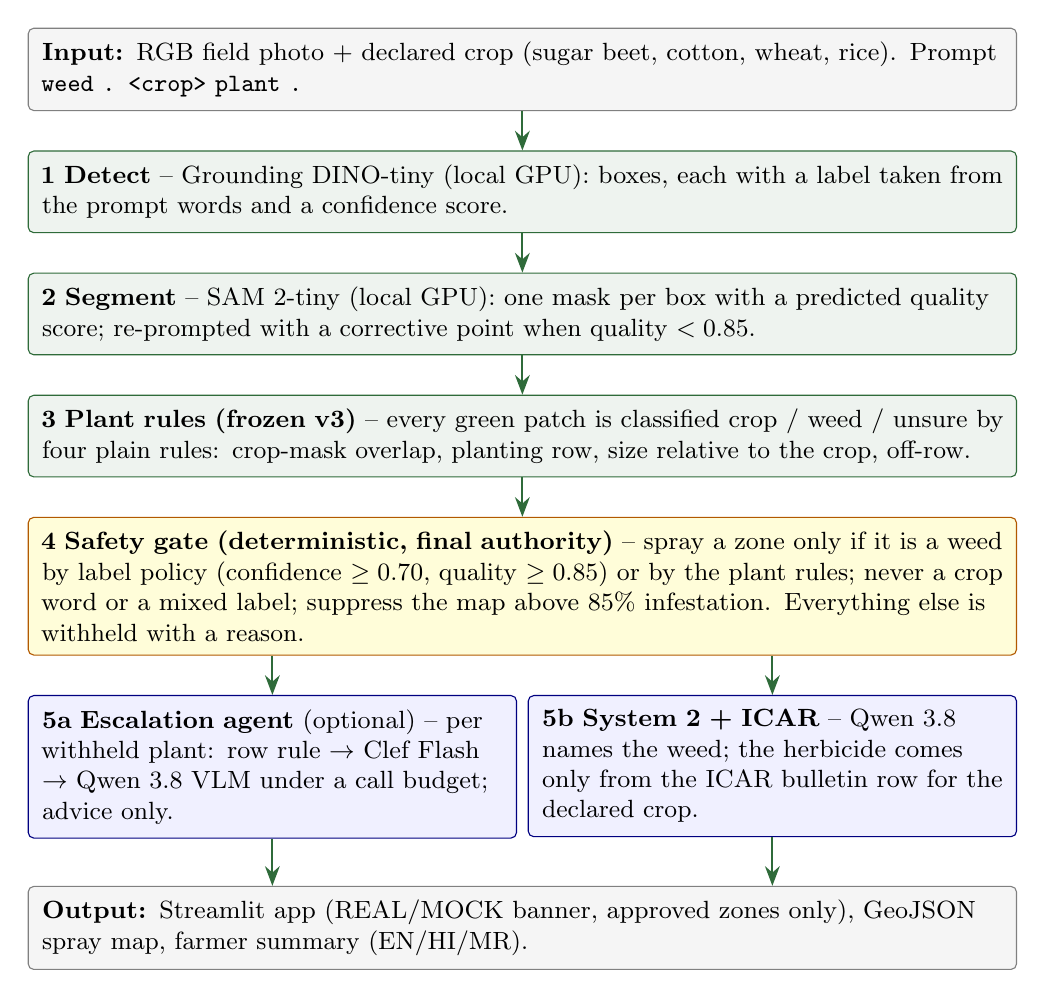
\begin{tikzpicture}[
  node distance=5mm,
  box/.style={draw=accent,rounded corners=2pt,fill=accent!8,text width=12.2cm,inner sep=5pt,font=\small,align=left},
  gate/.style={box,fill=yellow!15,draw=orange!70!black},
  cloud/.style={box,fill=blue!6,draw=blue!50!black,text width=5.85cm},
  io/.style={box,fill=black!4,draw=black!50},
  arr/.style={-{Stealth[length=2.5mm]},thick,accent}]
\node[io] (in) {\textbf{Input:} RGB field photo + declared crop (sugar beet, cotton, wheat, rice). Prompt \code{weed . <crop> plant .}};
\node[box,below=of in] (det) {\textbf{1 Detect} -- Grounding DINO-tiny (local GPU): boxes, each with a label taken from the prompt words and a confidence score.};
\node[box,below=of det] (seg) {\textbf{2 Segment} -- SAM~2-tiny (local GPU): one mask per box with a predicted quality score; re-prompted with a corrective point when quality $<0.85$.};
\node[box,below=of seg] (rules) {\textbf{3 Plant rules (frozen v3)} -- every green patch is classified crop / weed / unsure by four plain rules: crop-mask overlap, planting row, size relative to the crop, off-row.};
\node[gate,below=of rules] (gate) {\textbf{4 Safety gate (deterministic, final authority)} -- spray a zone only if it is a weed by label policy (confidence $\ge 0.70$, quality $\ge 0.85$) or by the plant rules; never a crop word or a mixed label; suppress the map above 85\% infestation. Everything else is withheld with a reason.};
\node[cloud,below=of gate.south west,anchor=north west] (agent) {\textbf{5a Escalation agent} (optional) -- per withheld plant: row rule $\rightarrow$ Clef Flash $\rightarrow$ Qwen~3.8 VLM under a call budget; advice only.};
\node[cloud,below=of gate.south east,anchor=north east] (sys2) {\textbf{5b System~2 + ICAR} -- Qwen~3.8 names the weed; the herbicide comes only from the ICAR bulletin row for the declared crop.};
\node[io,below=of agent.south west,anchor=north west,yshift=-1mm] (out) {\textbf{Output:} Streamlit app (REAL/MOCK banner, approved zones only), GeoJSON spray map, farmer summary (EN/HI/MR).};
\draw[arr] (in) -- (det); \draw[arr] (det) -- (seg); \draw[arr] (seg) -- (rules); \draw[arr] (rules) -- (gate);
\draw[arr] (gate.south -| agent.north) -- (agent.north); \draw[arr] (gate.south -| sys2.north) -- (sys2.north);
\draw[arr] (agent.south) -- (agent.south |- out.north); \draw[arr] (sys2.south) -- (sys2.south |- out.north);
\end{tikzpicture}
\caption{AgriAgent pipeline. Green: local, deterministic or pretrained; yellow: the safety gate; blue: cloud models that advise only.}\label{fig:arch}
\end{figure}

\section{The safety gate}\label{sec:gate}
The gate is the only component allowed to approve a spray zone (modules
\code{deterministic\_\allowbreak router.py} and \code{workflow.py}). Its rules are deliberately plain so that each can be unit tested and
explained; Section~\ref{sec:math-gate} states them as equations.
\begin{itemize}
\item \textbf{Label policy.} A detector mask is a spray candidate only if its label names a weed.
  Labels that name the crop, or mix crop and weed words (Grounding DINO sometimes returns ``weed sugar
  beet plant''), are withheld.
\item \textbf{Confidence and quality.} The detector score must be at least 0.70 and SAM~2's predicted
  mask quality at least 0.85. The application's slider may raise the confidence floor, never lower it.
\item \textbf{Not one plant.} A mask covering more than half of the photo is withheld: it is the whole
  field, not a weed.
\item \textbf{Infestation ceiling.} If approved zones cover more than 85\% of the photo, the whole map
  is suppressed.
\item \textbf{Plant-rule zones.} Patches the plant rules call ``weed'' are approved after every crop
  pixel has been removed from them; ``unsure'' patches never are.
\item \textbf{Fail safe.} Any exception, missing input or missing evidence results in withholding,
  never spraying.
\end{itemize}
An early version passed confidence and quality to the gate hard-coded as 1.0, so every ``weed'' was
sprayed; the bug was found in our code review and fixed before any measurement.

\section{Plant rules (v3, frozen)}\label{sec:rules}
Grounding DINO rarely boxes the small weeds: in our sugar beet photos it boxes mostly the large crop
plants (Section~\ref{sec:cheap}). Its boxes therefore cannot be the only spray candidates. The plant
rules (\code{src/vision/plant\_candidates.py}) take every connected patch of vegetation, found by
thresholding the excess-green index~\cite{woebbecke1995color} with a per-photo Otsu
threshold~\cite{hamuda2016survey} after closing small gaps between the leaves of one plant, and
classify it, in this order:
\begin{enumerate}
\item \textbf{crop} if at least 30\% of the patch lies inside a SAM~2 mask that the detector labelled as the crop;
\item \textbf{crop} if the photo shows clear planting rows and the patch lies on a dense row band;
\item \textbf{weed} if the photo has crop masks and the patch is smaller than a quarter of the median
  crop plant in the same photo (self-calibrating; no threshold was tuned on labels), otherwise
  \textbf{unsure};
\item \textbf{weed} if the photo has no crop masks but clear rows, and the patch lies off the row band;
\item \textbf{unsure} otherwise, which is never sprayed.
\end{enumerate}
Rules 2 and 4 use the row structure in the same spirit as the row-based labelling of Bah et
al.~\cite{bah2018unsupervised} and Louargant et al.~\cite{louargant2018rowcrops}. The rules were developed
on the 30 development photos and then frozen as ``v3'' before a single run on the 90 held-out photos.
Rule~4 is also the main known weakness (finding F1, Section~\ref{sec:f1}).

\section{The escalation agent}\label{sec:agent}
The only agent in AgriAgent (\code{src/agents/escalation\_agent.py}) reviews plants the gate withheld,
largest first, up to three per photo. For each plant it gathers evidence from the cheapest source to
the most expensive: the row rule, then Cloudflare's Clef Flash decision model~\cite{doc_cloudflare},
then the Qwen~3.8 27B vision-language model shown a crop of the plant. It stops when the evidence is
decisive or its call budget is spent. A source's stated confidence is not its accuracy, so each answer
is weighted by the source's accuracy measured on 20 labelled patches, and the answers are combined as
in a naive Bayes classifier (Section~\ref{sec:math-agent}). One source alone can never reach a
verdict; two that agree can; sources that disagree cancel out to ``unsure''. The agent returns a trace
of every call, so each verdict can be explained, and its verdict is advice: the gate still decides.

\section{System~2 and ICAR herbicide advice}
When the detections are uncertain, or when the user asks, System~2 shows the photo to Qwen~3.8 27B and
asks for the crop, the weed and the growth stage. The herbicide then comes only from a table
transcribed from the ICAR--DWR bulletin \emph{Herbicide Use in Indian Agriculture}~\cite{choudhury2016icar}
(\code{src/agronomy/knowledge\_store.py}), and only from the row for the declared crop and a matching
weed. Doses are clamped to the bulletin's maximum, and banned, withdrawn and refused herbicides (bulletin
Table~3.3) are rejected. If no row matches, the screen says ``no evidence'' instead of guessing. Every
row was checked against the PDF (Section~\ref{sec:icar}).

\section{Farmer summary}
A short plain-language summary is built only from the pipeline's own facts (zones sprayed, plants left
unsure, the prescription). A language model may reword it in Hindi or Marathi, with a fixed glossary
for crop and weed names. It is rejected, and the English template shown, if it fails or mentions a
dose when no prescription exists. Safety sentences (the wrong-crop warning and ``this is a suggestion,
read the label'') are fixed translated text appended after the model's wording, never left to the
model.

\section{Datasets}\label{sec:datasets}
\begin{table}[H]
\centering
\caption{Data sources and links.}\label{tab:datasets}
\begin{small}
\begin{tabularx}{\textwidth}{@{}L{3.1cm}YL{2.6cm}@{}}
\toprule
\textbf{Dataset} & \textbf{Contents and link} & \textbf{Used for}\\
\midrule
sugarbeets\-And\-weeds \cite{data_sugarbeets} & 120 photos, 512$\times$512, Pascal VOC boxes for sugar beet and weed. The images resemble the Bonn sugar beet data~\cite{chebrolu2017sugarbeet}; the uploader does not document the origin. \url{https://www.kaggle.com/datasets/wangyongkun/sugarbeetsandweeds} & 30 development + 90 held-out photos\\
Cotton\-Weed\-Det3 \cite{data_cottonweeddet3,rahman2023cotton} & Cotton field photos with boxes for three weeds (palmer amaranth, morningglory, waterhemp); cotton itself is never labelled. \url{https://www.kaggle.com/datasets/yuzhenlu/cottonweeddet3} & 8 development photos\\
ICAR--DWR bulletin No.~22~\cite{choudhury2016icar} & Approved herbicides per crop with dose, water volume and waiting period; list of banned herbicides. \url{https://dwr.icar.gov.in} & System~2 knowledge store\\
\bottomrule
\end{tabularx}
\end{small}
\end{table}

\section{Technology stack and hardware}
\begin{table}[H]
\centering
\caption{Technology stack.}\label{tab:stack}
\begin{small}
\begin{tabularx}{\textwidth}{@{}lY@{}}
\toprule
\textbf{Layer} & \textbf{Choice}\\
\midrule
Language & Python 3.11--3.13; type hints checked with mypy; style with ruff.\\
Vision models & \code{IDEA-Research/grounding-dino-tiny} and \code{facebook/sam2-hiera-tiny} through Hugging Face Transformers~\cite{doc_transformers}; PyTorch 2.11 with CUDA 12.8.\\
Reasoning models & Qwen~3.8 27B (\code{@cf/qwen/qwen3.8-27b}) and Clef Flash on Cloudflare Workers AI (free tier)~\cite{doc_cloudflare}; Groq~\cite{doc_groq} as an alternative provider.\\
Application & Streamlit~\cite{doc_streamlit}; GeoJSON export~\cite{rfc7946}.\\
Testing and CI & Python \code{unittest}; Streamlit \code{AppTest} for headless application tests; GitHub Actions on Python 3.11 and 3.13.\\
Hardware & Laptop with an NVIDIA RTX~5050 (8~GB) and 15~GB RAM. Both vision models together peak at about 2.4~GB of GPU memory; the system was also tested on an RTX~3050 (4~GB).\\
\bottomrule
\end{tabularx}
\end{small}
\end{table}

\section{Code structure}
\begin{table}[H]
\centering
\caption{Main modules.}\label{tab:modules}
\begin{small}
\begin{tabularx}{\textwidth}{@{}>{\raggedright\arraybackslash\footnotesize}p{6.2cm}Y@{}}
\toprule
\textbf{Module} & \textbf{Responsibility}\\
\midrule
\code{src/vision/grounding\_dino.py} & Detector wrapper: prompt to boxes; mock mode for tests; fails loudly if real weights cannot load.\\
\code{src/vision/sam2\_wrapper.py} & Boxes to masks with predicted quality; corrective-point refinement.\\
\code{src/vision/model\_cache.py} & Loads each real model once per process under a lock.\\
\code{src/vision/plant\_candidates.py} & Plant rules v3 (Section~\ref{sec:rules}).\\
\code{src/workflow.py} & \code{VisionWorkflowRunner}: detect, segment, refine, spray map with the gate, triage, System~2.\\
\code{src/agents/\allowbreak deterministic\_\allowbreak router.py} & Safety gate rules.\\
\code{src/agents/escalation\_agent.py} & Escalation agent and its three evidence sources.\\
\code{src/agronomy/} & System~2 reasoner, ICAR knowledge store, prescription and dose ceilings, providers, farmer summary.\\
\code{src/evaluation/} & Metrics: crop pixels sprayed, weed recall, savings, IoU/Dice; benchmark runner.\\
\code{app/} & Streamlit dashboard, KPI cards, visualisation, GeoJSON export.\\
\code{scripts/} & Baseline runner, manifest builders, provider check, verification and release scripts.\\
\code{tests/} & 235 unit tests and 35 end-to-end tests.\\
\bottomrule
\end{tabularx}
\end{small}
\end{table}

\section{Real and mock modes}
Every model wrapper has a mock mode that returns deterministic synthetic output, so that the
application and the tests run on any laptop without the 1.5~GB of weights. Early in the project, a
failed model load silently switched to mock output, and the application presented a mock diagnosis as
``verified''. Both were fixed: a real run that cannot load a model now raises an error, and every
result screen carries a REAL or MOCK banner. Mock mode never calls a cloud model.

\section{Application}
The Streamlit dashboard (\code{app/app.py}) takes a photo upload, the crop, the prompt, the confidence
slider (0.70 or higher), the nozzle buffer in pixels and two switches: force System~2, and review
unsure plants with the escalation agent (real mode, off by default). It shows the REAL/MOCK banner, a
wrong-crop warning when no plant matched the declared crop, KPI cards (area sprayed, herbicide saved,
zones), the photo beside the spray map with approved zones filled and outlined, the System~2 report,
the farmer summary and a GeoJSON download. An optional view colours every plant by the decision
taken: red sprayed, green protected as crop, yellow left alone (Figure~\ref{fig:verdict}). The last
result is cached against the photo and the settings, so changing the summary language or downloading
does not rerun the models.

\begin{figure}[H]
\centering
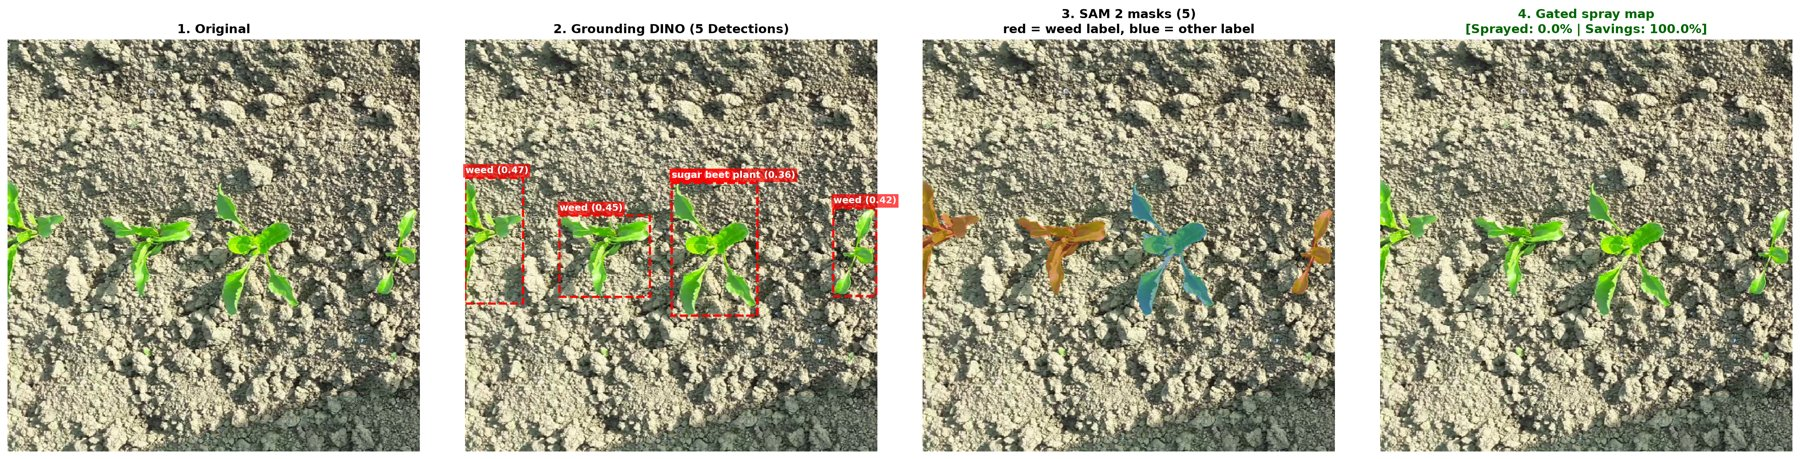
\includegraphics[width=0.95\textwidth]{real_run_beet_after_gate_fix}
\caption{Real run on a sugar beet photo (17 October, after the gate fix): photo, detector boxes, masks
and the spray map. All detector confidences were 0.36--0.47, below the 0.70 gate, so nothing was
sprayed: the crop is safe, but the weeds are missed. This is the Grounded SAM baseline behaviour that
the plant rules address.}\label{fig:gate}
\end{figure}

\begin{figure}[H]
\centering
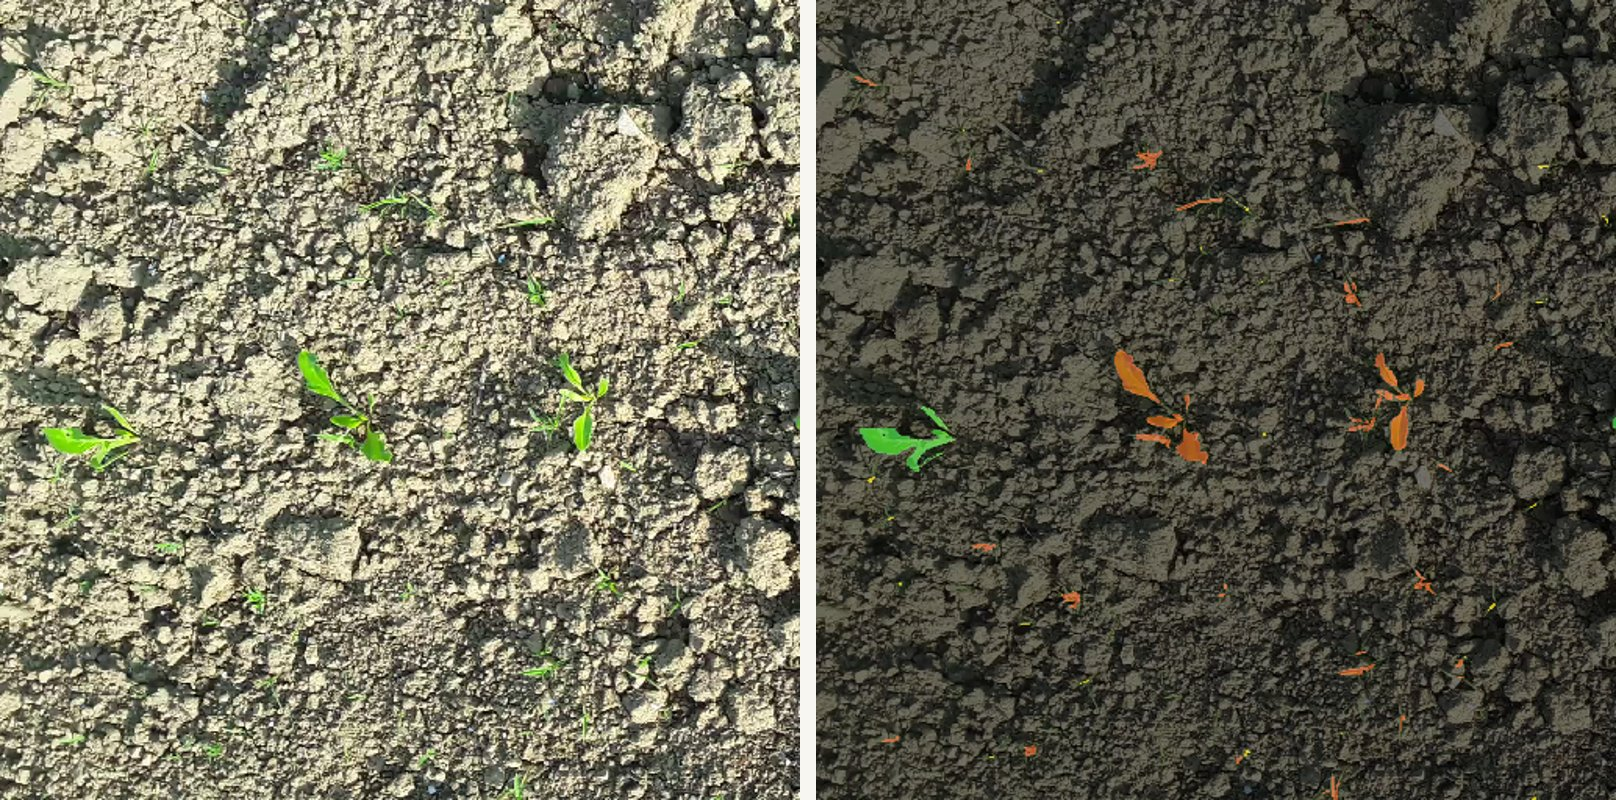
\includegraphics[width=0.49\textwidth]{verdict_beet_X2-30-0}\hfill
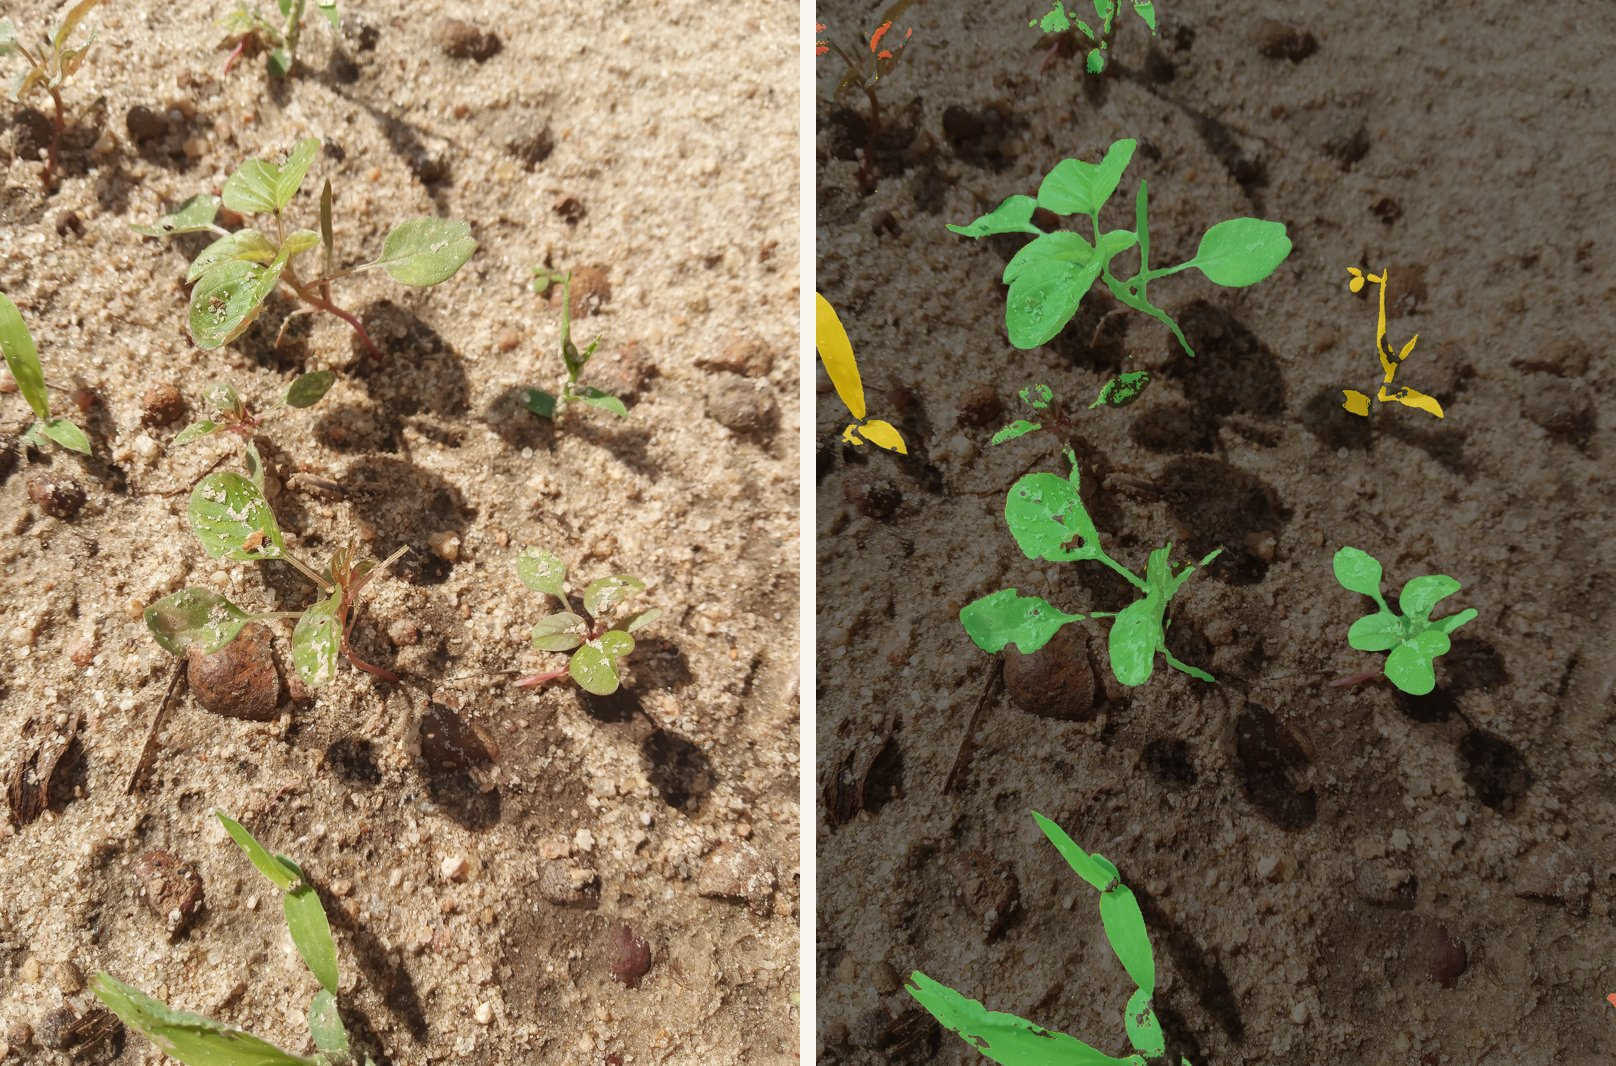
\includegraphics[width=0.49\textwidth]{verdict_cotton_CM_17}
\caption{The application's verdict view: red sprayed, green protected as crop, yellow left alone.
Left: sugar beet X2-30-0, where two of the three beets (centre and right) are wrongly sprayed; whole-beet
errors of this kind are analysed in Section~\ref{sec:f1}. Right: cotton CM\_17, where the detector boxed the large weeds as cotton,
so they were protected.}\label{fig:verdict}
\end{figure}

\section{GeoJSON export}
Each approved zone becomes one MultiPolygon feature traced along the exact pixel boundary of its mask,
with holes kept. Fragments under 16 pixels are dropped (jagged mask edges once produced 1,394 features
for three weeds). The top-left corner of the photo is pinned to a placeholder point at VJTI and each
pixel is taken as 5~mm on the ground; image rows grow downward and latitude northward, so rows are
subtracted. The file's metadata states that the coordinates are not GPS. Herbicide fields appear only
when System~2 produced a real prescription.

\chapter{Mathematical Model, Results and Analysis}\label{ch:results}

This chapter first states the system as a mathematical model (Section~\ref{sec:math}), exactly as the
code computes it, then the evaluation method (Section~\ref{sec:evalmethod}), the results with their
analysis (Sections~\ref{sec:baseline}--\ref{sec:speed}) and the testing (Section~\ref{sec:testing}).
All runs used the real models on the laptop GPU; each table names its source file in
\code{docs/results/} or \code{docs/testing/}.

\section{Mathematical model}\label{sec:math}

\subsection{Notation}
A photo is a map $I:\Omega\to[0,255]^3$ on the pixel grid $\Omega=\{1,\dots,H\}\times\{1,\dots,W\}$,
with channels $R,G,B$. For a set of pixels $A\subseteq\Omega$, $|A|$ is its number of pixels.
$B_r$ is the square structuring element of side $2r+1$; $\oplus$ and $\ominus$ are morphological
dilation and erosion.

\subsection{Vegetation mask}\label{sec:math-veg}
The excess-green index of Woebbecke et al.~\cite{woebbecke1995color} is computed per pixel,
\begin{equation}
  \mathrm{ExG}(p) = 2G(p) - R(p) - B(p), \qquad p\in\Omega .
\end{equation}
Its threshold $\tau^\ast$ is chosen per photo by Otsu's method: for a candidate threshold $t$ let
$\omega_0(t),\omega_1(t)$ be the fractions of pixels below and above $t$ and $\mu_0(t),\mu_1(t)$ their
mean ExG. The threshold maximises the between-class variance,
\begin{equation}
  \tau^\ast = \arg\max_t\; \sigma_b^2(t) = \arg\max_t\; \omega_0(t)\,\omega_1(t)\,\bigl(\mu_0(t)-\mu_1(t)\bigr)^2 ,
\end{equation}
and the vegetation mask is $V=\{p\in\Omega : \mathrm{ExG}(p) > \tau^\ast\}$.

\subsection{Plant patches}
Leaves of one plant are often separated by a few pixels, so gaps are closed before connected
components are taken:
\begin{equation}
  V' = (V \oplus B_r)\ominus B_r,\qquad r=\max\bigl(1,\operatorname{round}(0.01\max(H,W))\bigr).
\end{equation}
The plant patches $P_1,\dots,P_n$ are the 8-connected components of $V'$, each restricted to real
vegetation ($P_k\leftarrow P_k\cap V$); patches with $|P_k|<12$ pixels are ignored.

\subsection{Crop reference and planting rows}
Let $M_1,\dots,M_m$ be the SAM~2 masks whose detector label names the crop (and no weed), with masks
covering more than half of the photo removed. Their union is $C=\bigcup_j M_j$, the crop overlap of a
patch is $o(P)=|P\cap C|/|P|$, and the typical crop size is the median
\begin{equation}
  \tilde m = \operatorname{median}_j\, |M_j\cap V| .
\end{equation}
For the rows, the vegetation is summed along each image axis, e.g.\ $h(y)=\sum_x V(x,y)$, and smoothed
with a 15-pixel moving average to $\tilde h$. The axis with the larger peakiness
$\pi=\max\tilde h/\overline{\tilde h}$ is the row direction, and the photo has \emph{clear rows} iff
$\pi\ge 2$. A patch with centroid coordinate $c(P)$ across the rows lies \emph{on the row} iff
$\tilde h\bigl(c(P)\bigr)\ge 0.5\max\tilde h$.

\subsection{Plant classifier}
The four rules of Section~\ref{sec:rules} form a piecewise function, evaluated top to bottom:
\begin{equation}\label{eq:rules}
f(P)=\begin{cases}
\text{crop}   & \text{if } o(P)\ge 0.3,\\
\text{crop}   & \text{else if rows} \wedge \text{on-row}(P),\\
\text{weed}   & \text{else if } C\neq\emptyset \wedge |P| < 0.25\,\tilde m,\\
\text{unsure} & \text{else if } C\neq\emptyset,\\
\text{weed}   & \text{else if rows} \wedge \neg\,\text{on-row}(P),\\
\text{unsure} & \text{otherwise.}
\end{cases}
\end{equation}
Note the fifth line: the off-row rule is reached only when the photo has \emph{no} crop mask
($C=\emptyset$). That is exactly the situation of finding F1 (Section~\ref{sec:f1}).

\subsection{Safety gate}\label{sec:math-gate}
Each detection $i$ has a box, a label $\ell_i$, a confidence $s_i$, a SAM~2 mask $M_i$ and a predicted
mask quality $q_i$. With $\mathcal W(\ell)$ true when the label names a weed and $\mathcal C(\ell)$ true
when it names the crop, the gate approves a detector mask iff
\begin{equation}
  g_i = \mathcal W(\ell_i)\wedge\neg\,\mathcal C(\ell_i)\wedge s_i\ge\theta_s\wedge q_i\ge\theta_q\wedge
        \frac{|M_i|}{|\Omega|}\le 0.5,\qquad \theta_s=0.70,\ \theta_q=0.85 .
\end{equation}
The plant-rule weed set is $W_r=\bigcup_{f(P)=\text{weed}}P\setminus(C\cup C_r)$, where $C_r$ is the
union of patches classified as crop, so the nozzle never fires over a crop pixel. The spray map and
the infestation are
\begin{equation}
  S_0=\bigcup_{i:\,g_i}M_i\;\cup\;W_r,\qquad \iota=\frac{|S_0|}{|\Omega|},\qquad
  S=\begin{cases}S_0 & \iota\le 0.85\\ \emptyset & \iota>0.85\end{cases}
\end{equation}
In the application, the nozzle footprint is $S\oplus B_b$ for a buffer of $b$ pixels (default 10).

\subsection{Escalation agent}\label{sec:math-agent}
Source $k$ answers ``weed'' or ``crop'' with stated confidence $c_k$; its accuracy $a_k$ was measured
on 20 labelled patches (row rule 0.65, Clef Flash 0.70, Qwen VLM 0.80). The probability that the
answer is right, and from it the probability of ``weed'', are
\begin{equation}
  r_k = a_k c_k + (1-a_k)(1-c_k),\qquad
  p_k=\begin{cases} r_k & \text{answer ``weed''}\\ 1-r_k & \text{answer ``crop''}\end{cases},
\end{equation}
clipped to $[0.02,0.98]$. Assuming the sources err independently, the odds multiply from even odds
(a naive Bayes combination):
\begin{equation}
  O=\prod_k\frac{p_k}{1-p_k},\qquad P(\text{weed})=\frac{O}{1+O},\qquad
  \text{verdict}=\begin{cases}\text{weed} & P\ge 0.85\\ \text{crop} & P\le 0.15\\ \text{unsure} & \text{otherwise.}\end{cases}
\end{equation}
Since $r_k\le a_k\le 0.80<0.85$, one source alone can never reach a verdict. Two agreeing sources can:
for Clef ($a=0.70$) and Qwen ($a=0.80$) both certain, $O=\frac{0.7}{0.3}\cdot\frac{0.8}{0.2}=9.33$ and
$P=0.90$. Two sources that disagree with equal strength cancel to $O=1$, $P=0.5$, ``unsure''.

\subsection{Evaluation metrics}\label{sec:math-metrics}
Labels are boxes, so ground truth is vegetation inside boxes. With crop boxes $\{b^c_j\}$ and weed
boxes $\{b^w_j\}$,
\begin{equation}
  G_c = V\cap\bigcup_j b^c_j,\qquad G_w=\Bigl(V\cap\bigcup_j b^w_j\Bigr)\setminus G_c .
\end{equation}
Summed over all photos of a set (pooled, not averaged per photo):
\begin{align}
  \text{Crop sprayed (\%)} &= 100\,\frac{\sum|S\cap G_c|}{\sum|G_c|} &&\text{(damage, lower is better)}\\
  \text{Weed recall (\%)}  &= 100\,\frac{\sum|S\cap G_w|}{\sum|G_w|} &&\text{(higher is better)}\\
  \text{Herbicide saved (\%)} &= 100\Bigl(1-\frac{\sum|S|}{\sum|\Omega|}\Bigr) &&\text{(against blanket spraying)}
\end{align}
At plant level, a crop plant $j$ is \emph{touched} if $|S\cap V\cap b^c_j|>0$, and a weed is \emph{hit}
if at least half its vegetation pixels are sprayed. For mask quality, the usual
$\mathrm{IoU}(A,B)=|A\cap B|/|A\cup B|$ and $\mathrm{Dice}(A,B)=2|A\cap B|/(|A|+|B|)$ are implemented.
The metric code has unit tests built from three hand-computed $5\times5$ grids, for example crop
$2/6=33.3\%$, weed recall $3/4=75\%$ and saving 80\%.

\subsection{Complexity}
Vegetation, closing, connected components and rows are each $O(HW)$; the rules add $O(n)$ for $n$
patches, so System~1's own logic is linear in the image size. Photos larger than 1024~px on the long
side are subsampled for the rules and the result is upsampled back. Run time is dominated by the two
neural networks (Section~\ref{sec:speed}).

\section{Evaluation method}\label{sec:evalmethod}

\subsection{A fabricated evaluation set, found and replaced}
The first evaluation set (\code{eval\_manifest\_v1}, 20 images) looked real but was a template: every
sugar beet image carried the same two crop and six weed boxes, and every cotton image a cotton box,
although the official cotton dataset labels no cotton at all. Only one or two of eight boxes per beet
image matched the official labels, and none per cotton image (Figure~\ref{fig:audit}). A metric
reported on it earlier was meaningless and was withdrawn. It was replaced by \code{eval\_manifest\_v2},
built by a script that copies boxes from the official XML files; rebuilding it from a fresh download
gives an identical manifest.

\begin{figure}[H]
\centering
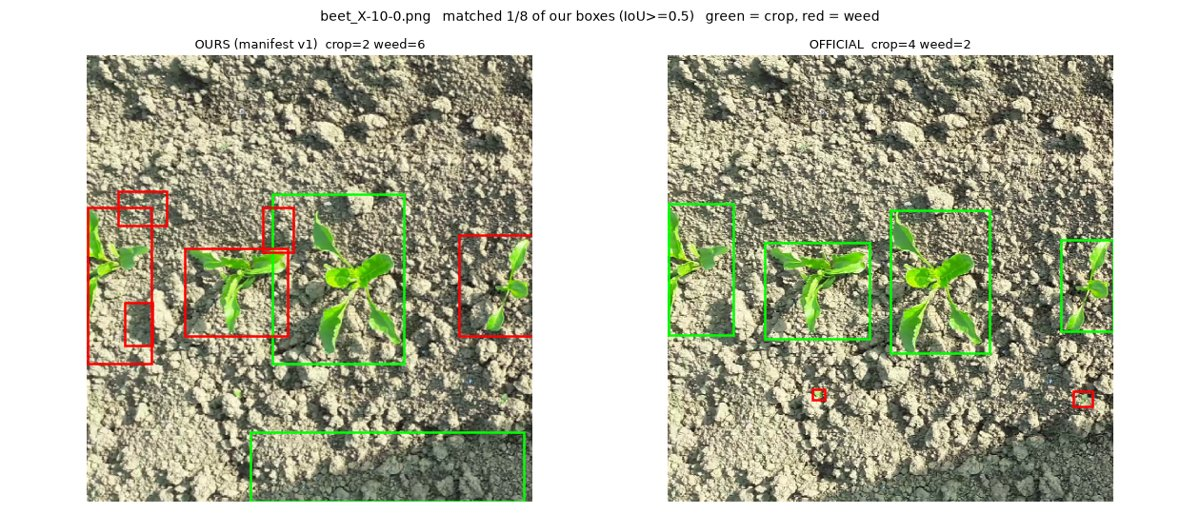
\includegraphics[width=0.49\textwidth]{audit_beet_X-10-0}\hfill
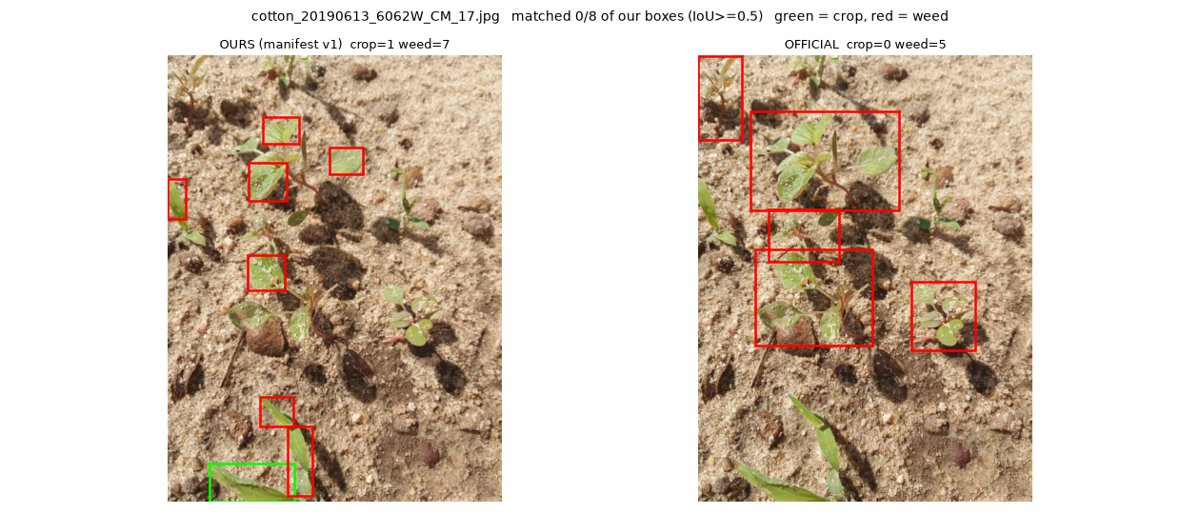
\includegraphics[width=0.49\textwidth]{audit_cotton_CM_17}
\caption{Label audit. Left: beet X-10-0, old labels put a ``crop'' box on bare soil and ``weed'' boxes on
beets. Right: cotton CM\_17, no old box matches the official weed boxes.}\label{fig:audit}
\end{figure}

\subsection{Development and held-out sets}
\begin{table}[H]
\centering
\caption{Evaluation sets. All labels are copied unchanged from the official files.}\label{tab:sets}
\begin{small}
\begin{tabularx}{\textwidth}{@{}L{4.3cm}L{2.1cm}L{3.1cm}Y@{}}
\toprule
\textbf{Set} & \textbf{Photos} & \textbf{Labels} & \textbf{Use}\\
\midrule
\code{eval\_manifest\_v2} (development) & 30 beet + 8 cotton & 93 beets, 282 weeds; 19 cotton weeds & Every design decision and every variant.\\
\code{eval\_manifest\_v2\_holdout} & 90 beet & 363 beets, 215 weeds & Run \textbf{once}, on 18 October, after the rules were frozen.\\
\bottomrule
\end{tabularx}
\end{small}
\end{table}
The held-out set is every sugar beet photo not in the development set. A repeat on 23 October
reproduced every number exactly, and a run of the first ten photos twice gave zero differences: the
pipeline is deterministic.

\subsection{Settings compared}
\begin{table}[H]
\centering
\caption{Settings compared. Prompt \code{weed . <crop> plant .}, detector box threshold 0.35, buffer 10~px.}\label{tab:settings}
\begin{small}
\begin{tabularx}{\textwidth}{@{}lY@{}}
\toprule
\textbf{Setting} & \textbf{Meaning}\\
\midrule
\code{every\_mask} & Spray every SAM~2 mask, whatever its label: the upper bound on recall and on damage.\\
\code{gate\_0.35}, \code{0.50}, \code{0.70} & Grounded SAM label policy with confidence floor $\theta_s$ = 0.35, 0.50 or 0.70 (0.70 is deployed).\\
\code{+exclusion} & Also subtract crop-labelled masks from weed masks before spraying.\\
\code{plant\_rules} & The deployed product: plant rules v3 plus the gate.\\
agent & Deployed gate plus the escalation agent reviewing up to three withheld plants per photo.\\
\bottomrule
\end{tabularx}
\end{small}
\end{table}

\section{Baseline: Grounded SAM label policy (RQ1)}\label{sec:baseline}
\begin{table}[H]
\centering
\caption{Sugar beet development set (30 photos).}\label{tab:baseline}
\begin{small}
\begin{tabularx}{\textwidth}{@{}L{4.3cm}RRRRR@{}}
\toprule
\textbf{Setting} & \textbf{Crop sprayed \%} & \textbf{Weed recall \%} & \textbf{Saved \%} & \textbf{Beets touched} & \textbf{Weeds hit}\\
\midrule
every\_mask & 93.9 & 97.6 & 39.3 & 87/93 & 265/282\\
gate\_0.35 & 70.8 & 9.0 & 93.0 & 45/93 & 7/282\\
gate\_0.50 & 20.5 & 6.8 & 98.0 & 8/93 & 1/282\\
gate\_0.70 (deployed) & 0.0 & 0.0 & 100.0 & 0/93 & 0/282\\
\bottomrule
\end{tabularx}
\end{small}
\src{docs/results/baseline_v2_20261018.md}
\end{table}

\textbf{Analysis.} SAM~2 outlines plants well: spraying every mask reaches 97.6\% weed recall. The
problem is the labels. At a confidence floor of 0.35 the label policy sprays 70.8\% of crop pixels
while hitting only 9\% of weed pixels: the detector calls crop plants ``weed'' more often than it
finds the real weeds. Real Grounding DINO scores on these photos never exceeded 0.68, so the deployed
gate at 0.70 sprays nothing at all: perfectly safe and perfectly useless. On cotton, spraying every
mask hits 75.8\% of weed pixels, but every gated setting hits 0\%. \textbf{Answer to RQ1:} text prompts
alone do not separate crop from weed on these photos; lowering the gate buys recall only by spraying
the crop. This agrees with Chong et al.~\cite{chong2025zeroshot}.

\section{Cheap additions: crop exclusion, thresholds, tiling (RQ3)}\label{sec:cheap}
\begin{table}[H]
\centering
\caption{Crop exclusion and detector variants, sugar beet development set.}\label{tab:cheap}
\begin{small}
\begin{tabularx}{\textwidth}{@{}L{5.0cm}RRRR@{}}
\toprule
\textbf{Setting} & \textbf{Crop sprayed \%} & \textbf{Weed recall \%} & \textbf{Beets touched} & \textbf{s / photo}\\
\midrule
gate\_0.35 & 70.8 & 9.0 & 45/93 & 0.58\\
gate\_0.35 + exclusion & 50.1 & 9.0 & 38/93 & 0.58\\
gate\_0.50 & 20.5 & 6.8 & 8/93 & 0.58\\
gate\_0.50 + exclusion & \textbf{5.3} & 6.8 & 2/93 & 0.58\\
box threshold 0.20, gate\_0.50 + exclusion & 0.0 & 0.4 & 0/93 & 1.03\\
$2\times2$ tiles, gate\_0.35 & 74.6 & 10.1 & 49/93 & 3.76\\
\bottomrule
\end{tabularx}
\end{small}
\src{docs/results/exclusion_v2_20261018.md, detector_variants_20261018.md}
\end{table}

\textbf{Analysis.} Subtracting crop masks from weed masks cut crop pixels sprayed from 20.5\% to 5.3\%
at a 0.50 floor with no loss of recall. Running the detector on $2\times2$ tiles, or with a lower box
threshold, finds more plants but labels them no better, and slows the pipeline up to 13 times. The
bottleneck is classification, not detection. Plant-sized SAM~2 masks from detector boxes covered only
about 9\% of the beet weed pixels; the 97.6\% of \code{every\_mask} comes largely from masks covering the
whole photo.

\section{Plant rules on the development set}
\begin{table}[H]
\centering
\caption{Plant rules v3, sugar beet development set.}\label{tab:rulesdev}
\begin{small}
\begin{tabularx}{\textwidth}{@{}L{4.3cm}RRRRR@{}}
\toprule
\textbf{Setting} & \textbf{Crop sprayed \%} & \textbf{Weed recall \%} & \textbf{Saved \%} & \textbf{Beets touched} & \textbf{Weeds hit}\\
\midrule
every\_plant\_mask & 84.7 & 9.1 & 91.6 & 53/93 & 8/282\\
gate\_0.50 + exclusion & 5.3 & 6.8 & 99.3 & 2/93 & 1/282\\
\textbf{plant\_rules (v3)} & \textbf{4.6} & \textbf{71.5} & 90.5 & 21/93 & 219/282\\
\bottomrule
\end{tabularx}
\end{small}
\src{docs/results/plant_rules_v3_20261018.md, pipeline_plant_rules_dev_20261020.md}
\end{table}

\section{Held-out result (the headline)}\label{sec:holdout}
\begin{table}[H]
\centering
\caption{Held-out sugar beet set (90 photos, evaluated once).}\label{tab:holdout}
\begin{small}
\begin{tabularx}{\textwidth}{@{}L{4.3cm}RRRRR@{}}
\toprule
\textbf{Setting} & \textbf{Crop sprayed \%} & \textbf{Weed recall \%} & \textbf{Saved \%} & \textbf{Beets touched} & \textbf{Weeds hit}\\
\midrule
every\_mask & 94.4 & 93.2 & 60.2 & 334/363 & 204/215\\
Grounded SAM, gate\_0.35 & 65.5 & 1.8 & 85.0 & 242/363 & 3/215\\
Grounded SAM, gate\_0.50 & 22.5 & 0.0 & 95.5 & 49/363 & 0/215\\
Grounded SAM, gate\_0.70 (deployed) & 0.0 & 0.0 & 100.0 & 0/363 & 0/215\\
gate\_0.50 + exclusion & 5.5 & 0.0 & 98.8 & 24/363 & 0/215\\
\textbf{plant\_rules (v3), the product} & \textbf{8.8} & \textbf{77.9} & 95.0 & 104/363 & 177/215\\
\bottomrule
\end{tabularx}
\end{small}
\src{docs/results/holdout_plant_rules_v3_20261018.md}
\end{table}

\begin{figure}[H]
\centering
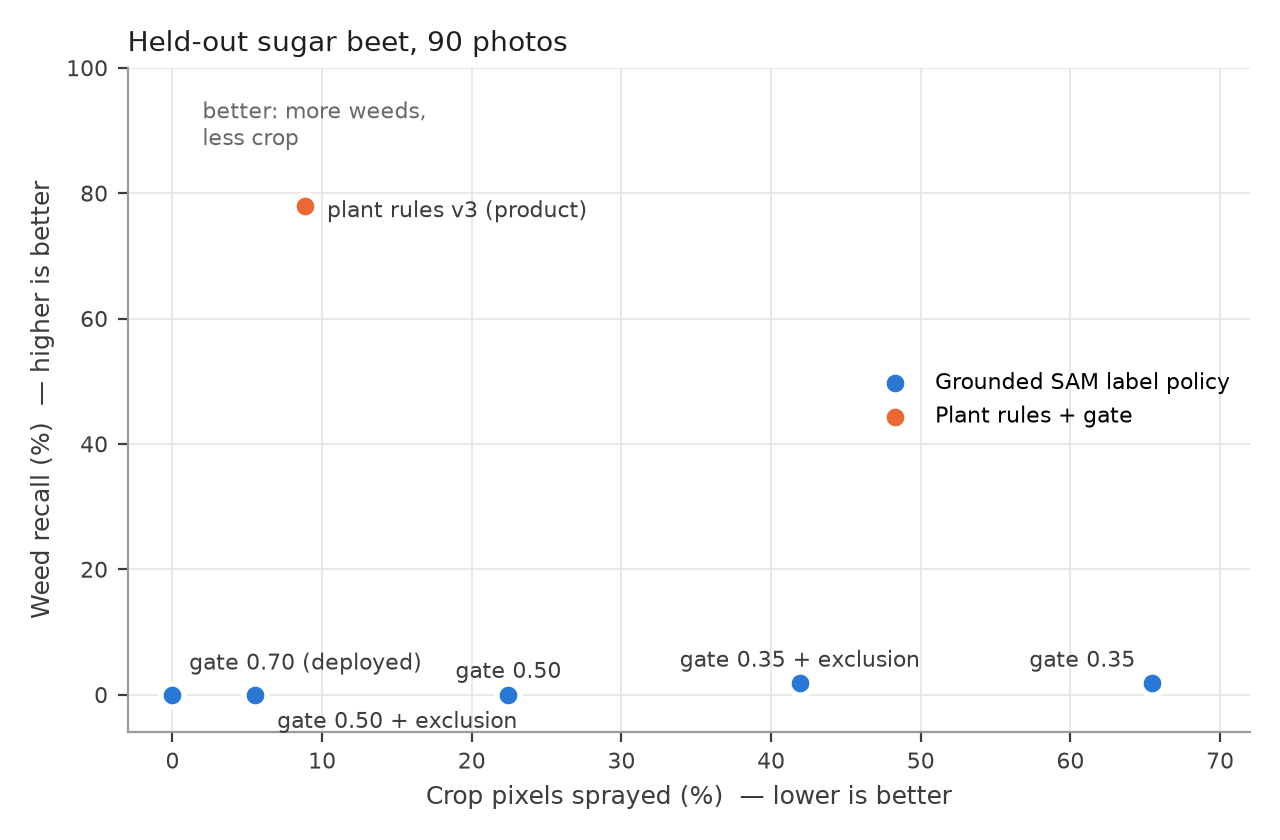
\includegraphics[width=0.78\textwidth]{tradeoff_holdout}
\caption{Crop pixels sprayed against weed recall on the held-out set. Every Grounded SAM setting lies on
the left edge (almost no weeds hit); the plant rules move the operating point to 77.9\% recall at 8.8\%
crop sprayed.}\label{fig:tradeoff}
\end{figure}

\textbf{Analysis.} On photos it had never seen, the product hits 77.9\% of weed pixels (177 of 215
weeds) and sprays 8.8\% of crop pixels, against 1.8\% and 65.5\% for the best-recall Grounded SAM
setting, while saving 95\% of the herbicide of blanket spraying. Held-out recall is higher than on the
development set (71.5\%), so there is no sign of overfitting the rules to the development photos. The
cost is real: 104 of 363 beets have at least one sprayed pixel, mostly small specks at a plant's edge,
but some whole plants (Section~\ref{sec:f1}). On the eight cotton photos the rules reach only 10.4\%
weed recall: rule~3 assumes weeds are smaller than the crop, true for young sugar beet and false for
cotton close-ups where one large weed fills the photo.

\textbf{Is a held-out set of 90 photos enough?} No model was trained or fine-tuned in this project, so
the 120 sugar beet photos are evaluation data only, and they are the complete public
dataset~\cite{data_sugarbeets}, not a sample from it. The held-out part contains 363 crop plants and
215 weeds. At plant level, the 95\% Wilson confidence interval for the share of weeds hit is
76.7--86.8\% (177/215) for the plant rules against 0.5--4.0\% (3/215) for the best-recall Grounded
SAM setting; for crop plants touched it is 24.2--33.5\% (104/363) against 61.7--71.3\% (242/363).
The intervals are far apart, so the size of the test set limits how precisely the numbers are known,
not the conclusion. What the data cannot show is generality beyond young sugar beet in one dataset,
which is why our claims are stated for that crop only.

\section{Escalation agent (RQ2)}\label{sec:agent-results}
\begin{table}[H]
\centering
\caption{Verdicts of the escalation agent on 69 withheld plants, development set, deployed gate.}\label{tab:agent}
\begin{small}
\begin{tabularx}{0.8\textwidth}{@{}YRRR@{}}
\toprule
\textbf{Plant really was} & \textbf{Agent: weed} & \textbf{Agent: crop} & \textbf{Agent: unsure}\\
\midrule
crop (44) & 0 & 13 & 31\\
weed (25) & 0 & 1 & 24\\
\bottomrule
\end{tabularx}
\end{small}
\src{docs/results/agent_v2_20261018.md}
\end{table}

\textbf{Analysis.} The agent reviewed up to three withheld plants per photo (69 in total, about 40
minutes; 14 of 69 Groq calls were lost to the free tier's per-minute limit and counted as ``no
answer''). It never approved spraying a crop plant, and 13 of its 14 ``crop'' verdicts were right. But
it called none of the 25 real weeds a weed, so the spray map was identical with and without it.
\textbf{Answer to RQ2:} escalation to vision-language models, combined conservatively, is safe and
precise but not effective for the crop-versus-weed decision on this data. The rules reach 77.9\%
recall with no model calls at all; the agent stays in the product, off by default, as a reviewer that
explains withheld plants.

\section{Vision-language models as a second opinion}
\begin{table}[H]
\centering
\caption{Crop-or-weed answers on 20 labelled plant patches (10 beet crop, 6 beet weed, 4 cotton weed).}\label{tab:vlm}
\begin{small}
\begin{tabularx}{\textwidth}{@{}YRRR@{}}
\toprule
\textbf{Source} & \textbf{Correct} & \textbf{Crop called crop} & \textbf{Weed called weed}\\
\midrule
Qwen~3.8 27B on Groq, told the crop & 16/20 & 9/10 & 7/10\\
Qwen~3.8 27B on Cloudflare, same prompt & 12/20 & 5/10 & 7/10\\
Clef Flash (Cloudflare) & 14/20 & 8/10 & 6/10\\
Row rule, no model & 13/20 & 7/10 & 6/10\\
\bottomrule
\end{tabularx}
\end{small}
\src{docs/results/t2_2_crop_or_weed_groq_20261017.json, qwen_provider_check_20261030.md}
\end{table}
Twenty patches is a small sample, but two lessons hold. First, the same model name gave 16 of 20 from
one provider and 12 of 20 from another (finding F25), so the agent's accuracy weights $a_k$ are tied to
the provider they were measured on. Second, in the sugar beet data the weeds are tiny (median 16~px
across) and the crops large (median 68~px), so size alone separates many cases; this is why rule~3
works on beet and not on cotton.

\section{Main limitation: rule 4 and whole beets (F1)}\label{sec:f1}
Rule~4 calls any off-row patch a weed whatever its size, and by Equation~\eqref{eq:rules} it applies
exactly when the detector found no crop. When photo X-10-0 was rotated by 90\textdegree, the detector
returned no crop box and the largest beet (4,410~px) was sprayed completely (Figure~\ref{fig:f1}). A
size limit on rule~4 was measured on the development set only:
\begin{table}[H]
\centering
\caption{The size limit trades recall for crop safety (development set).}\label{tab:f1}
\begin{small}
\begin{tabularx}{\textwidth}{@{}YRRR@{}}
\toprule
\textbf{Rule 4 applies up to \ldots{} $\times$ the median on-row plant} & \textbf{Crop sprayed \%} & \textbf{Weed recall \%} & \textbf{Beets mostly sprayed}\\
\midrule
0.25 & 0.25 & 12.9 & 0\\
1.0 & 0.98 & 31.3 & 3\\
1.5 & 1.20 & 39.1 & 4\\
no limit (v3, frozen) & 4.55 & 71.5 & 11\\
\bottomrule
\end{tabularx}
\end{small}
\src{scripts/experiment_f1_row_rule.py; docs/testing/Verification_Report_20261023.md}
\end{table}
Rule~4 gives most of the recall and most of the damage. We kept v3 frozen, because no unused held-out
set is left to test a changed rule fairly, and report the trade-off; a ``safe mode'' with the size limit
is future scope.

\begin{figure}[H]
\centering
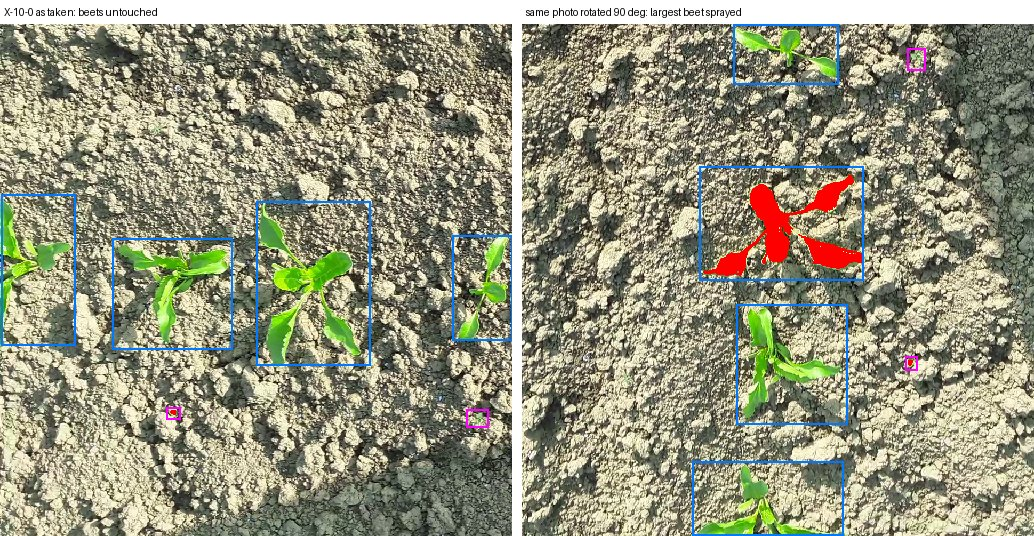
\includegraphics[width=0.85\textwidth]{verify_rotation_X-10-0}
\caption{Finding F1. Photo X-10-0 rotated by 90\textdegree: the detector returns no crop box, so rule~4
marks the largest beet as an off-row weed and it is sprayed completely.}\label{fig:f1}
\end{figure}

\section{ICAR herbicide table check}\label{sec:icar}
Every herbicide row and dose ceiling in the code was compared with the rendered pages of the
bulletin~\cite{choudhury2016icar} (\code{docs/results/icar\_table\_check\_20261020.md}). Eight cotton rows
were correct; two had a missing value stored as 0 instead of ``not stated''. The rice row for
pyrazosulfuron-ethyl was dangerous: 20~g a.i./ha with a 75-day waiting period, against the bulletin's
10--15~g and 95 days, an overdose with a shorter waiting period. It and six other values were
corrected, and all nine banned, withdrawn and refused herbicides matched. Regression tests fail on the
old values. In a manual test on cotton photo CM\_17, System~2 named the weed \emph{Amaranthus} (correct
genus) and matched a real ICAR cotton row: pyrithiobac-sodium 10\% EC, 75~g a.i./ha, waiting period 160
days, bulletin page 35.

\section{Speed}\label{sec:speed}
The pipeline takes 0.56--0.64~s per photo on the RTX~5050 after the first photo (detection 0.21~s,
segmentation 0.27--0.37~s), inside NFR3. Loading both models takes 4--14~s and happens once per
application process. A real run in the application, including the cloud diagnosis, takes about 15~s,
or about 40~s with the escalation agent. On the 4~GB RTX~3050 of the second test cycle the first real
run took 3.6~s.

\section{Testing}\label{sec:testing}
\begin{table}[H]
\centering
\caption{Testing summary.}\label{tab:testing}
\begin{small}
\begin{tabularx}{\textwidth}{@{}L{3.2cm}YL{3.0cm}@{}}
\toprule
\textbf{Level} & \textbf{What} & \textbf{Result}\\
\midrule
Unit & 235 tests: gate rules, plant rules, metrics (hand-computed grids), ICAR rows vs bulletin, GeoJSON geometry, providers, farmer summary, model cache, verdict view. & all pass\\
End to end & 35 tests through the workflow and the app in mock mode. & all pass\\
Static & ruff, ruff format, mypy on \code{src/}. & clean\\
CI & GitHub Actions on every push, Python 3.11 and 3.13. & green\\
System cycle 0 (16 Oct) & 16 app test cases on a fresh Windows install (Amit Ingle). & 7 pass, 9 fail $\rightarrow$ 8 issues, all fixed\\
Headless regression & The app driven by Streamlit AppTest in mock and real mode. & all pass\\
Verification run (23 Oct) & Fresh clone, data rebuild, held-out reproduction, determinism, 12 edge-case images, no-network run. & reproduces exactly; 13 findings\\
Manual cycle (30 Oct) & MT-01 \ldots{} MT-10 on six test photos, real mode. & core cases pass; 16 findings\\
System cycle 2 (7--8 Nov) & Final build on Windows~11, Python 3.13, RTX~3050 (4~GB), real mode: install, automated checks, regression of F24--F29, manual and exploratory cases (Amit Ingle). & 24/24 executed cases pass; 1 finding (F30)\\
\bottomrule
\end{tabularx}
\end{small}
\end{table}

\begin{small}
\begin{longtable}{@{}L{1.4cm}L{1.4cm}L{7.6cm}L{3.0cm}@{}}
\caption{Selected findings (full lists: \code{docs/testing/Verification\_Report\_20261023.md}, \code{Manual\_Test\_Cycle\_20261030.md}).}\label{tab:findings}\\
\toprule
\textbf{ID} & \textbf{Severity} & \textbf{Finding} & \textbf{Status}\\
\midrule\endfirsthead
\toprule
\textbf{ID} & \textbf{Severity} & \textbf{Finding} & \textbf{Status}\\
\midrule\endhead
F1 & high & Rule 4 sprays large off-row beets when the detector misses the crop box. & measured; limitation\\
F2 & medium & Unpinned dependencies resolved to untested versions. & fixed: lock file\\
F3 & medium & Groq free-tier rate limit (429) on back-to-back runs. & fixed: Cloudflare, agent off by default\\
F14--F16 & medium & GeoJSON upside down; buffer labelled cm but in pixels; 1.1~m per pixel. & fixed\\
F18 & high & Wrong crop setting: no crop masks, so rule 4 sprays crop plants. & fixed: warning\\
F20 & medium & Every click reran the models. & fixed: result cache\\
F22 & medium & Full-size photos sent to the cloud model (12,349 tokens). & fixed: resized\\
F23 & medium & Hindi summary called sugar beet ``sweet potato''. & fixed: glossary\\
F25 & info & Qwen 16/20 on Groq vs 12/20 on Cloudflare. & reported\\
F26 & medium & Intermittent ``Cannot copy out of meta tensor'' when a rerun interrupted model loading. & fixed: load once under a lock\\
F29 & medium & Hindi summary turned the ICAR suggestion into an instruction and dropped ``read the label''. & fixed: fixed-text caveat\\
F30 & info & On a screenshot of a text document Grounding DINO reported a ``sugar beet plant'' at 0.71. & safe: crop labels are never sprayed\\
\bottomrule
\end{longtable}
\end{small}

In the first system test cycle a team member installed the project from scratch on Windows and ran
16 application test cases; the nine failures (GitHub issues \#5--\#12) included an app crash on start,
herbicide fields in GeoJSON with System~2 off, an empty prompt silently replaced by a default that
invented weeds, an unapplied confidence slider, mock diagnoses shown as ``verified'' and a cotton
herbicide recommended for other crops. Each was reproduced, fixed, covered by a test, re-run with the
tester's exact steps and closed with its cause. In the second cycle the final build passed all 24
executed cases on a different machine, including the exploratory case that produced F30: Grounding DINO
labelled a page of text ``sugar beet plant'' at 0.71 confidence, and the gate sprayed nothing because
the label names the crop, a small illustration of RQ1. The final build is tagged \code{v1.0.0}.

\chapter{Conclusion}\label{ch:conclusion}

\section{Answers to the research questions}
\begin{itemize}
\item \textbf{RQ1.} Grounded SAM's text labels do not separate crop from weed: on held-out photos
  65.5\% of crop pixels are sprayed for 1.8\% weed recall, and the deployed 0.70 gate sprays nothing.
  SAM~2's masks are good; the labels are the problem.
\item \textbf{RQ2.} The escalation agent is safe (no crop approved) and precise (13 of 14 crop
  verdicts right) but adds no weed recall (0 of 25 weeds).
\item \textbf{RQ3.} Crop exclusion cuts damage without a recall gain; lower thresholds and tiling do
  not help. Plain rules on crop overlap, rows and relative size give the best trade-off measured:
  8.8\% crop sprayed and 77.9\% weed recall on held-out photos.
\end{itemize}

\section{Relation to the base paper and the closest work}
We implemented the Grounded SAM pipeline~\cite{ren2024groundedsam} and confirm on field photos the
weakness that Chong et al.~\cite{chong2025zeroshot} argue for: text prompts are ill-defined for crop
and weed. We do not claim to beat WaW's 12.1\% weed IoU, because we measure a different quantity
(sprayed vegetation inside labelled boxes, not pixel IoU against pixel masks) on different data. What
we add is the sprayer's view: how much crop lands on the map, how many weeds are hit, and how far a
transparent, deterministic safety layer moves that trade-off without training.

\section{What we learned, including what went wrong}\label{sec:lessons}
\begin{enumerate}
\item \textbf{AI-written status claims.} AI-generated documents early in the project described
  intentions as facts: ``100\% complete'', 227 tests (there were 175), a ``0.99 IoU'' that was SAM~2's
  own confidence score. Since 11 October every claim carries a status label (REAL, PARTIAL, MOCK,
  PLANNED) and a command output.
\item \textbf{Fabricated labels.} The first evaluation set was a template. Ground truth is now copied
  from the official files by a script and audited.
\item \textbf{Fabricated references.} An early bibliography contained papers that do not exist. Every
  journal and proceedings reference in this report is now generated from its Crossref record.
\item \textbf{Silent fake output.} Failed model loads became mock output; every SAM~2 mask got an
  invented quality of 0.88; the reasoning model never received the photo. Real mode now fails loudly.
\item \textbf{A gate that ignored its inputs.} Confidence and quality were passed as 1.0. Each gate
  rule now has a test with real values.
\item \textbf{Measure before claiming.} The original proposal promised ``over 70\% chemical saving''
  and ``under 40~ms''. Neither was measured then; the measured numbers are in
  Chapter~\ref{ch:results}.
\end{enumerate}

\section{Limitations}
\begin{itemize}
\item Evaluation data: the complete public sugar beet set (120 photos; 90 held out with 363 crop and
  215 weed plants) from one source of undocumented origin, and 8 cotton photos. No training data is
  used, by design; the results are therefore claimed for young sugar beet only (confidence intervals in
  Section~\ref{sec:holdout}).
\item Box labels only, so the pixel metrics are approximate (vegetation inside boxes).
\item The plant rules exploit ``weeds are smaller than the crop'', true for young sugar beet; they
  reach only 10.4\% weed recall on cotton.
\item Finding F1: whole off-row beets can be sprayed when the detector misses the crop box (104 of 363
  held-out beets touched, mostly specks).
\item The held-out set has been used, so any changed rule can only be tested on new data.
\item Coordinates are not GPS; no sprayer, latency or field trial was tested.
\item Cloud reasoning depends on free tiers and on the provider (F25).
\end{itemize}

\section{Conclusion}
AgriAgent shows, with official labels and a held-out set, that a zero-shot Grounded SAM pipeline cannot
on its own tell a weed from a crop plant well enough to spray: it either sprays the crop or nothing. A
small set of transparent rules and a deterministic safety gate, with no training and no model calls,
move the held-out result to 77.9\% weed recall at 8.8\% crop pixels sprayed and a 95\% herbicide saving,
in 0.6~s per photo on a laptop. A vision-language escalation agent, used conservatively, stays safe but
does not add recall. The system is honest about what it is: a research prototype that measures how far
zero-shot vision gets on this problem, not a product for real spraying.

\chapter{Future Scope}\label{ch:future}

\begin{enumerate}
\item \textbf{A like-for-like comparison with WaW.} Run the pipeline on the PhenoBench validation
  set~\cite{weyler2024phenobench} (pixel labels) and report weed IoU, the metric of Chong et
  al.~\cite{chong2025zeroshot}.
\item \textbf{Species-aware features instead of text labels.} Replace the detector's words with
  BioCLIP~\cite{stevens2024bioclip} features of each plant, as WaW does, and keep the safety gate on
  top.
\item \textbf{A ``safe mode'' for rule 4.} Limit the off-row rule by plant size (Table~\ref{tab:f1}),
  tested on new held-out data, so that a missed crop box can no longer cause a whole crop plant to be sprayed.
\item \textbf{Few-shot adaptation.} Adapt the detector with a handful of labelled field photos, as
  Singh et al.~\cite{singh2025fewshot} suggest, and measure how many labels close the gap to supervised
  detectors~\cite{rahman2023cotton,dang2023yoloweeds}.
\item \textbf{Using the row over time.} Exploit image sequences along the row~\cite{lottes2018fcn,lottes2020stem}
  and automatically labelled inter-row weeds~\cite{bah2018unsupervised} to calibrate the rules per field.
\item \textbf{Farmer-facing agent and interface.} A conversational assistant over the same verified
  facts, in Indian languages, on a mobile-first web interface.
\item \textbf{Real deployment.} GPS from drone or sprayer metadata, nozzle latency, a field trial with
  an agronomist, and the other applications of the original proposal (disease, yield, canopy cover,
  nutrient stress).
\end{enumerate}


\cleardoublepage
\phantomsection
\markboth{References}{References}
\renewcommand{\bibname}{References}
\bibliographystyle{IEEEtran}
\bibliography{references_manual,references_crossref}

\appendix
\chapter{How to Run}\label{app:run}
The commands below install AgriAgent from the public repository, download the two models, and run the
application, one photo, the measurements and the tests.

\begin{lstlisting}[language=bash]
git clone https://github.com/Chaitanya-666/agriAgent && cd agriAgent
python3.11 -m venv .venv && source .venv/bin/activate        # Python 3.11-3.13
pip install -r requirements-lock.txt && pip install -e . --no-deps
python scripts/download_models.py          # Grounding DINO-tiny + SAM 2-tiny
cp .env.example .env                        # add CLOUDFLARE_ACCOUNT_ID, CLOUDFLARE_API_TOKEN
streamlit run app/app.py                    # dashboard
PYTHONPATH=. python -m unittest discover -s tests            # tests
python scripts/run_baseline.py --manifest data/manifests/eval_manifest_v2_holdout.json
\end{lstlisting}
The release \code{v1.0.0} is at \url{https://github.com/Chaitanya-666/agriAgent/releases/tag/v1.0.0}.

\chapter{Team Roles}\label{app:contrib}
The project was planned in four tracks: (1) vision pipeline, workflow and safety gate, (2) agronomy and
herbicide advice, (3) data and evaluation, (4) application, testing and release. The table records
each member's role in the work as delivered.

\begin{small}
\begin{longtable}{@{}L{3.2cm}L{11.2cm}@{}}
\caption{Roles of the team members.}\label{tab:roles}\\
\toprule
\textbf{Member} & \textbf{Role and work}\\
\midrule\endfirsthead
\toprule
\textbf{Member} & \textbf{Role and work}\\
\midrule\endhead
Chaitanya Shinde (team lead) & Research questions, scope and methodology; the vision pipeline (Grounding DINO, SAM~2, refinement, model loading); the deterministic safety gate and spray map; plant rules v3; the escalation agent; the final System~2 and ICAR knowledge store, checked row by row against the bulletin; farmer summary; the Streamlit application and GeoJSON export; the evaluation sets, label audit and metrics; all experiments in Chapter~\ref{ch:results}; the unit and end-to-end tests, CI, verification run and manual test cycle; fixes for findings F1--F30; this report and the presentation.\\[4pt]
Amit Ingle & The first Streamlit dashboard; system test cycle~0 (16 cases on a fresh Windows installation, 8 issues filed); system test cycle~2 on the final build (24 of 24 cases passed on Windows~11 with an RTX~3050), including install, regression and exploratory cases; the packaging bug report; the \code{v1.0.0} release (version bump, release notes, draft release); the live demonstration.\\[4pt]
Sumant Vetal & The first version of the System~2 agronomy module (diagnosis and herbicide advice), later rewritten and integrated.\\[4pt]
Sahil Chavan & The dataset downloader used to fetch the public datasets.\\
\bottomrule
\end{longtable}
\end{small}


\end{document}
